\section{Апробация моделей на экспериментальных данных}
	Для апробации разработанных моделей выберем результаты измерений на интергральной 
	схеме 1564ЛЕ1, состоящие из трёх частотных сканов, полученных при температурах 
	263~К, 283~К, 303~К. К сожалению, полученные частотные сканы содержат относительно 
	немного точек: 340, 340 и 34, соответственно. Поскольку требуется только 
	идентификация параметров модели, а не вычисление сигнала DLTS по новым значениям 
	частоты опорной функции, предлагается отказаться от оценки идентифицированной 
	модели на тестовом наборе, и ограничиться только оценками корня из 
	среднеквадратической ошибки (RMSE) на тренировочных данных и кросвалидацией.

	В данном разделе приводятся схема подключения образца, условия эксперимента,
	результаты измерений (частотные сканы), результаты идентификации частотных сканов
	разными моделями и их сравнение, а также анализ графиков Аррениуса, построенных 
	по вычисленным параметрам моделей.

	\subsection{Экспериментальные данные}
	\emph{Цель исследования}: регистрация частотных сканов интегральной схемы
	1564ЛЕ1 №1 в двухполюсном включении при разных температурах. Схема 
	подключения с эквивалентным диодом показана на рисунке~\ref{pic:scheme}. 

	\begin{figure}[!ht]
		\centering
		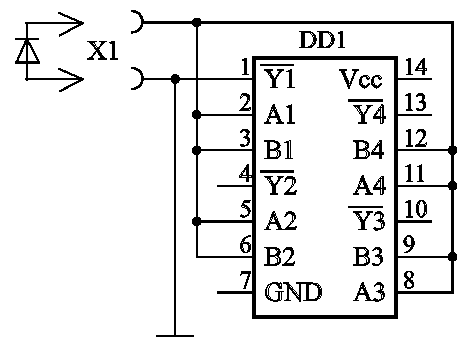
\includegraphics[width=0.4\textwidth]{scheme}
		\caption{Схема двухполюсного включения ИС 1564ЛЕ1.}
		\label{pic:scheme}
	\end{figure}

	Условия, одинаковые для всех сканов перечислены в таблице 
	\ref{table:common_conditions}. Графики с результатфми измерений 
	предствалены на рисунках \ref{pic:train_data_263}, \ref{pic:train_data_283}
	и \ref{pic:train_data_303}.

	\begin{table}[!ht]
		\centering
		\caption{Условия, одинаковые для всех сканов.}
		\begin{tabular}{|l|l|}
			\hline
			Параметр                           & Значение             \\ \hline
			Образцы                            & 1564ЛЕ1~№1           \\ \hline
			Длительность импульса              & 10                   \\ 
			заполнения, мкс                    &                      \\ \hline
			$U_1$                              & -4 В                 \\ \hline
			$U_r$                              & -5 В                 \\ \hline
			Автоматическая компенсация моста   & включена             \\ \hline
			Начальная частота сканирования, Гц & 1                    \\ \hline
			Конечная  частота сканирования, Гц & 2500                 \\ \hline
			Направление сканирования           & вниз по частоте      \\ \hline
			Интервал между измерениями, с      & 3.5                  \\ \hline
			Постоянная интегрирования, с       & 3                    \\ \hline
		\end{tabular}
		\label{table:common_conditions}
	\end{table}

	\begin{figure}[!htp]
		\centering
		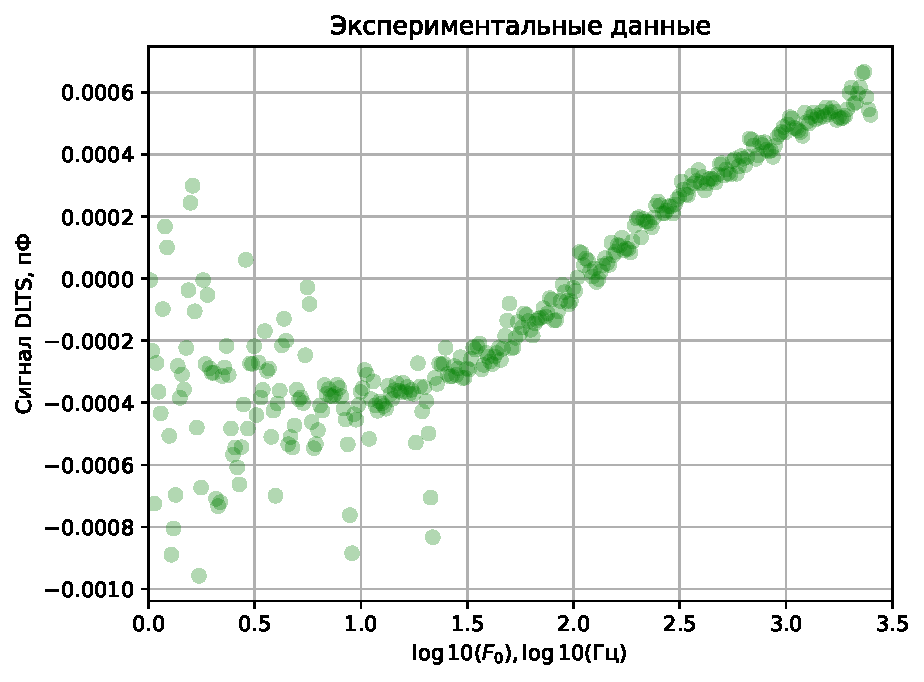
\includegraphics[width=0.5\textwidth]{1564ЛЕ1№1_п1_2500Гц-1Гц_1пФ_-10С_-4В-5В_10мВ_10мкс_шаг_0,01_train_data}
		\caption{Частотный скан, полученный при температуре 263 К.}
		\label{pic:train_data_263}
	\end{figure}

	\begin{figure}[!htp]
		\centering
		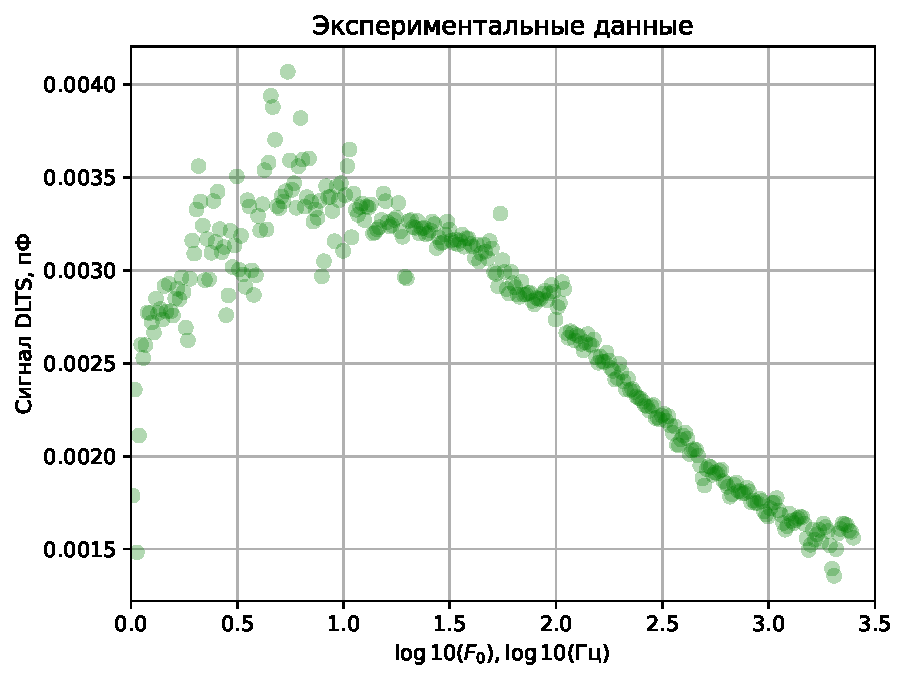
\includegraphics[width=0.5\textwidth]{1564ЛЕ1№1_п1_2500Гц-1Гц_1пФ_+10С_-4В-5В_50мВ_10мкс_шаг_0,01_train_data}
		\caption{Частотный скан, полученный при температуре 283 К.}
		\label{pic:train_data_283}
	\end{figure}

	\begin{figure}[!htp]
		\centering
		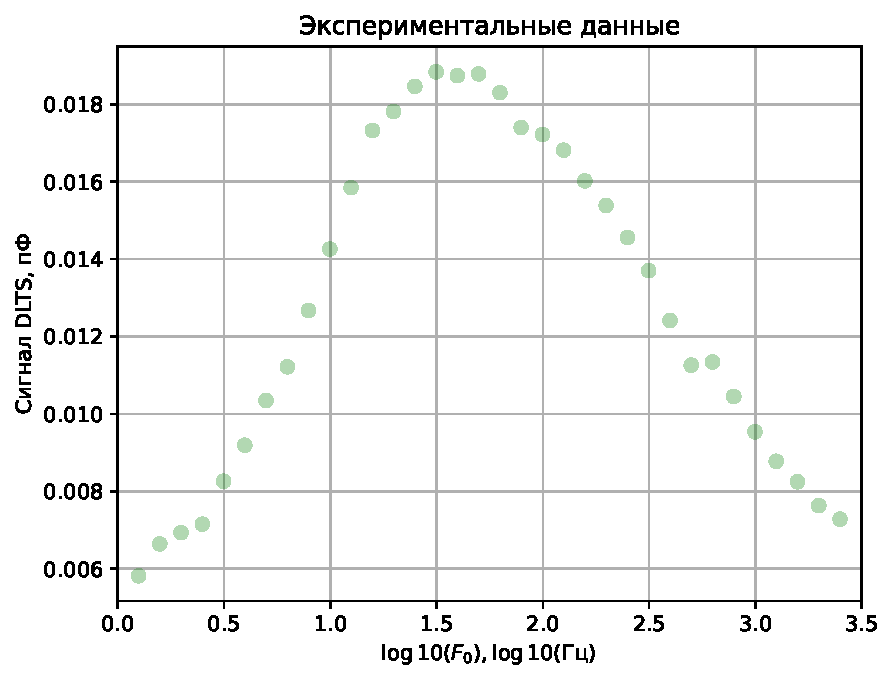
\includegraphics[width=0.5\textwidth]{1564ЛЕ1№1_п1_2500Гц-1Гц_10пФ_+30С_-4В-5В_50мВ_10мкс_шаг_0,1_train_data}
		\caption{Частотный скан, полученный при температуре 303 К.}
		\label{pic:train_data_303}
	\end{figure}


	\newpage
	\subsection{Частотный скан при температуре 263 К}
	\subsubsection{Моноэкспоненциальная модель с показателем $p$}

	Как показано на рисунке \ref{pic:train_data_263}, частотный скан имеет два
	пика: положительный и отрицательный, поэтому сначала выполним идентификацию
	модели с показателем $p$ с начальными параметрами близкими к положительному
	пику. Результат идентификации представлен на рисунке 
	\ref{pic:model_monoexp_p_positive_263}.

	\begin{figure}[!htp]
		\centering
		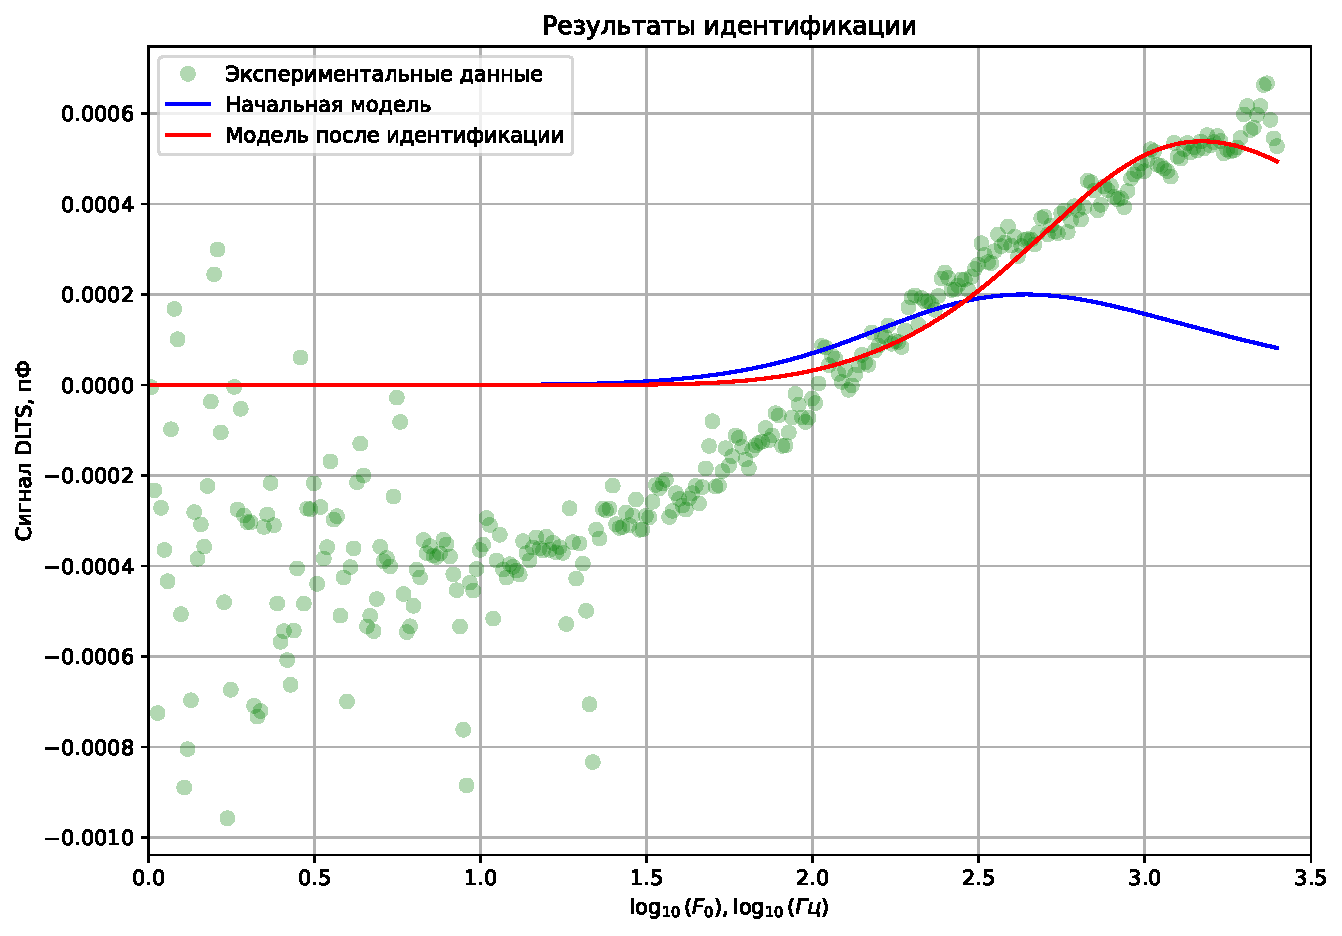
\includegraphics[width=0.75\textwidth]{1564ЛЕ1№1_п1_2500Гц-1Гц_1пФ_-10С_-4В-5В_10мВ_10мкс_шаг_0,01_single_exp_model_1}
		\caption{Результат идентификации положительного пика частотного скана
		         при $T=263K$.}
		\label{pic:model_monoexp_p_positive_263}
	\end{figure}

	Для того, чтобы убедиться, что алгоритм идентификации достиг минимума 
	функции потерь, построим график значений среднеквадратической ошибки на 
	каждой итерации, график нормируем оносительно максимального значения метрики.
	Получившийся график представлен на рисунке \ref{pic:loss_monoexp_p_positive_263}.

	\begin{figure}[!htp]
		\centering
		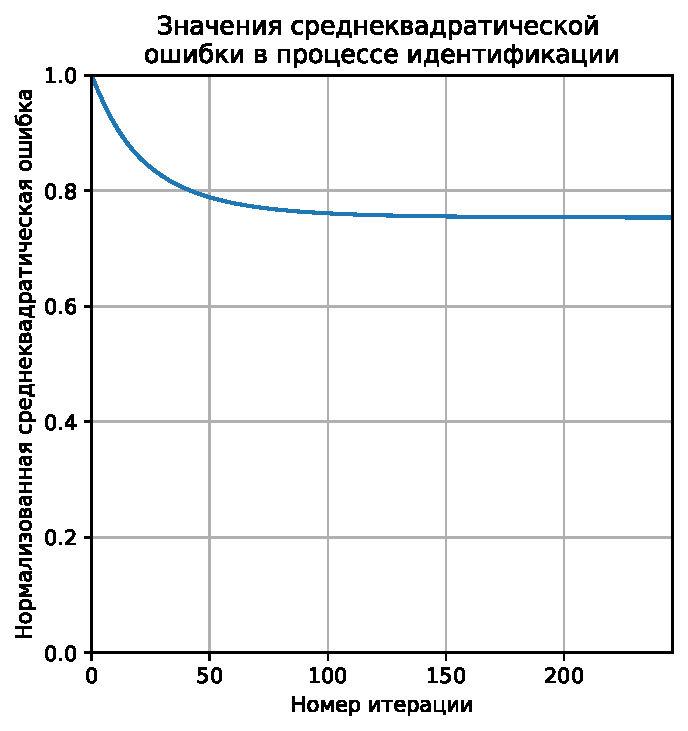
\includegraphics[width=0.35\textwidth]{1564ЛЕ1№1_п1_2500Гц-1Гц_1пФ_-10С_-4В-5В_10мВ_10мкс_шаг_0,01_single_exp_model_loss_1}
		\caption{График среднеквадратической ошибки в процессе идентификации,
		         нормированной относительно её максимального значения.}
		\label{pic:loss_monoexp_p_positive_263}
	\end{figure}

	График среднеквадратической ошибки выходит на <<плато>>, что свидетельствует 
	о том, что решение сошлось, однако довольно высокое значение 
	среднеквадратической ошибки может указывать на то, что алгоритм нашёл 
	локальный минимум функции потерь.

	Построим график отклонений результатов моделирования от экспериментальных 
	данных (рисунок \ref{pic:deviations_monoexp_p_positive_263}), чтобы оценить 
	систематическую ошибку.

	\begin{figure}[!htp]
		\centering
		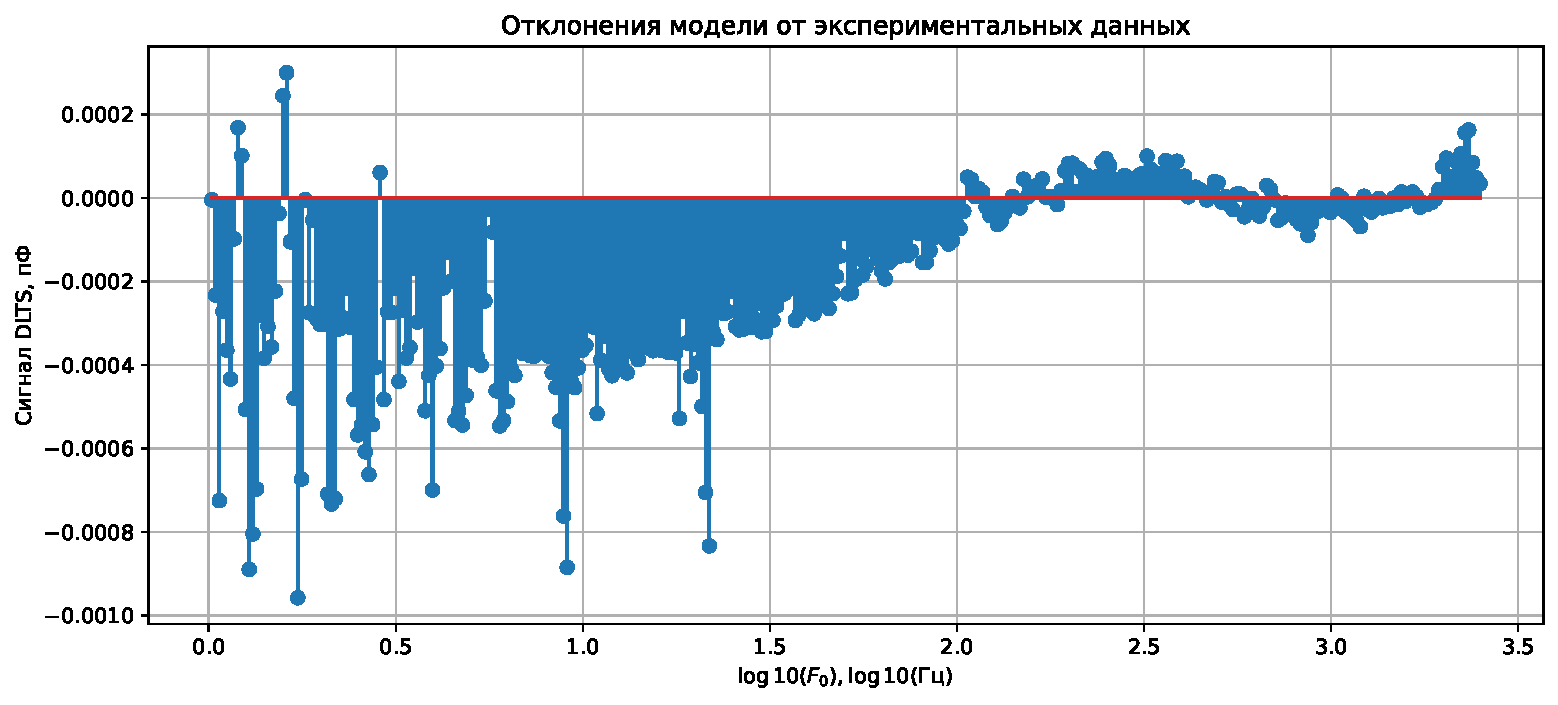
\includegraphics[width=0.75\textwidth]{1564ЛЕ1№1_п1_2500Гц-1Гц_1пФ_-10С_-4В-5В_10мВ_10мкс_шаг_0,01_single_exp_deviations_1}
		\caption{График отклонений результатов, полученных на идентифицированной
		модели, от экспериментальных данных.}
		\label{pic:deviations_monoexp_p_positive_263}
	\end{figure}

	Рисунки \ref{pic:model_monoexp_p_positive_263} и 
	\ref{pic:deviations_monoexp_p_positive_263} демонстрируют, что модель не 
	охватывает половину частотного скана с отрицательными значениями сигнала
	DLTS, что закономерно для однопиковой модели.

	Построим гистограму распределения отклонений резульатов моделирования от
	экспериментальных данных. В идеальном случае данное распределение должно
	стремиться к распределению погрешностей измерительного прибора и быть близко
	к нормальному распределению, в данном случае (рисунок 
	\ref{pic:hist_monoexp_p_positive_263}) это не так. На рисунке 
	\ref{pic:hist_monoexp_p_positive_263} сплошной линией показан результат
	сглаживания гистограммы c гаусовым усредняющим ядром (в англоязычной 
	литературе данный алгоритм называется <<kernel density estimation>>).

	\begin{figure}[!htp]
		\centering
		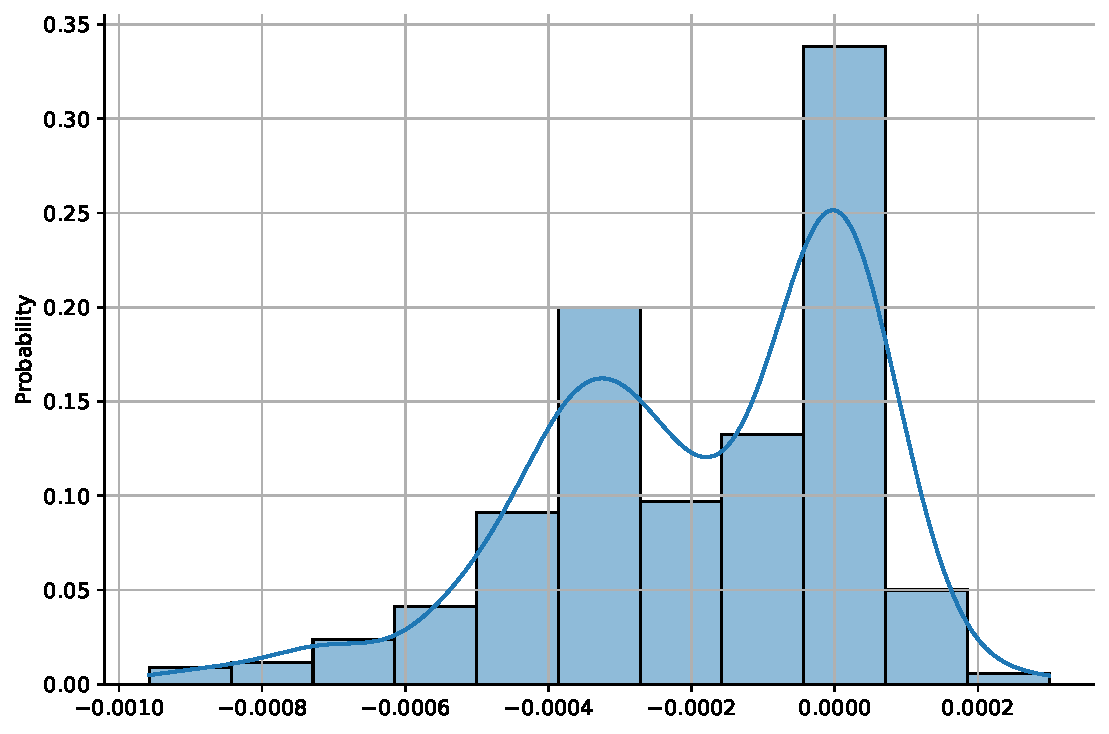
\includegraphics[width=0.5\textwidth]{1564ЛЕ1№1_п1_2500Гц-1Гц_1пФ_-10С_-4В-5В_10мВ_10мкс_шаг_0,01_single_exp_hist_1}
		\caption{Гистограмма отклонений данных, полученных на идентифицированной 
		         модели, от экспериментальных данных. Сплошной линией показан 
		         результат сглаживания гистограммы.}
		\label{pic:hist_monoexp_p_positive_263}
	\end{figure}

	В таблице \ref{table:results_monoexp_p_positive_263} приведём параметры 
	идентифицированной модели и результаты оценок точности моделирования.

	\begin{table}[!htp]
    	\centering
    	\caption{Результаты идентификации модели}
		\begin{tabular}{|l|l|}
			\hline
			Параметр                           & Значение  \\ \hline
			Постоянна времени $\tau$, с        & 0,000286  \\ \hline
			Амплитуда, пФ                      & 0.000538  \\ \hline
			Показатель $p$                     & 0.802     \\ \hline
			Результат кросвалидации (RMSE), пФ & 0.000290  \\ \hline
			RMSE, пФ                           & 0.000291  \\ \hline
		\end{tabular}
		\label{table:results_monoexp_p_positive_263}
	\end{table}

	Построим полученный спектр частотного скана (рисунок 
	\ref{pic:spectr_monoexp_p_positive_263}), чтобы предствить
	результаты в более наглядной форме.

	\begin{figure}[!htp]
		\centering
		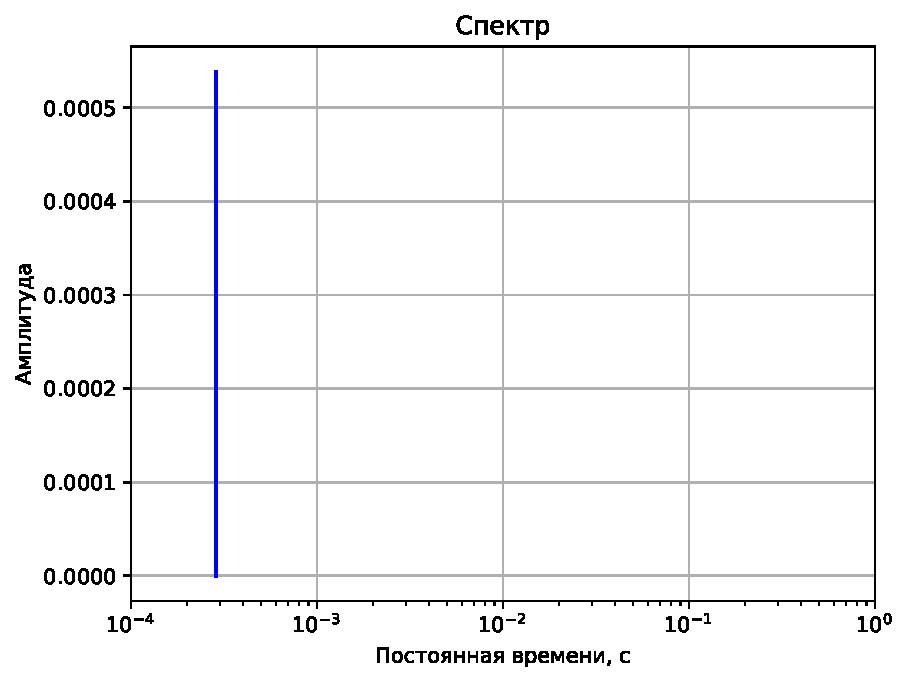
\includegraphics[width=0.5\textwidth]{1564ЛЕ1№1_п1_2500Гц-1Гц_1пФ_-10С_-4В-5В_10мВ_10мкс_шаг_0,01_single_exp_spectr_1}
		\caption{Спектр сигнала релаксации ёмкости. Амплитуда указана в пФ.}
		\label{pic:spectr_monoexp_p_positive_263}
	\end{figure}

	Идентифицируем эту же модель с начальными параметрами близкими к параметрам
	отрицательного пика. На рисунке \ref{pic:model_monoexp_p_negative_263}
	представлен график с результатами идентификации.

	\begin{figure}[!htp]
		\centering
		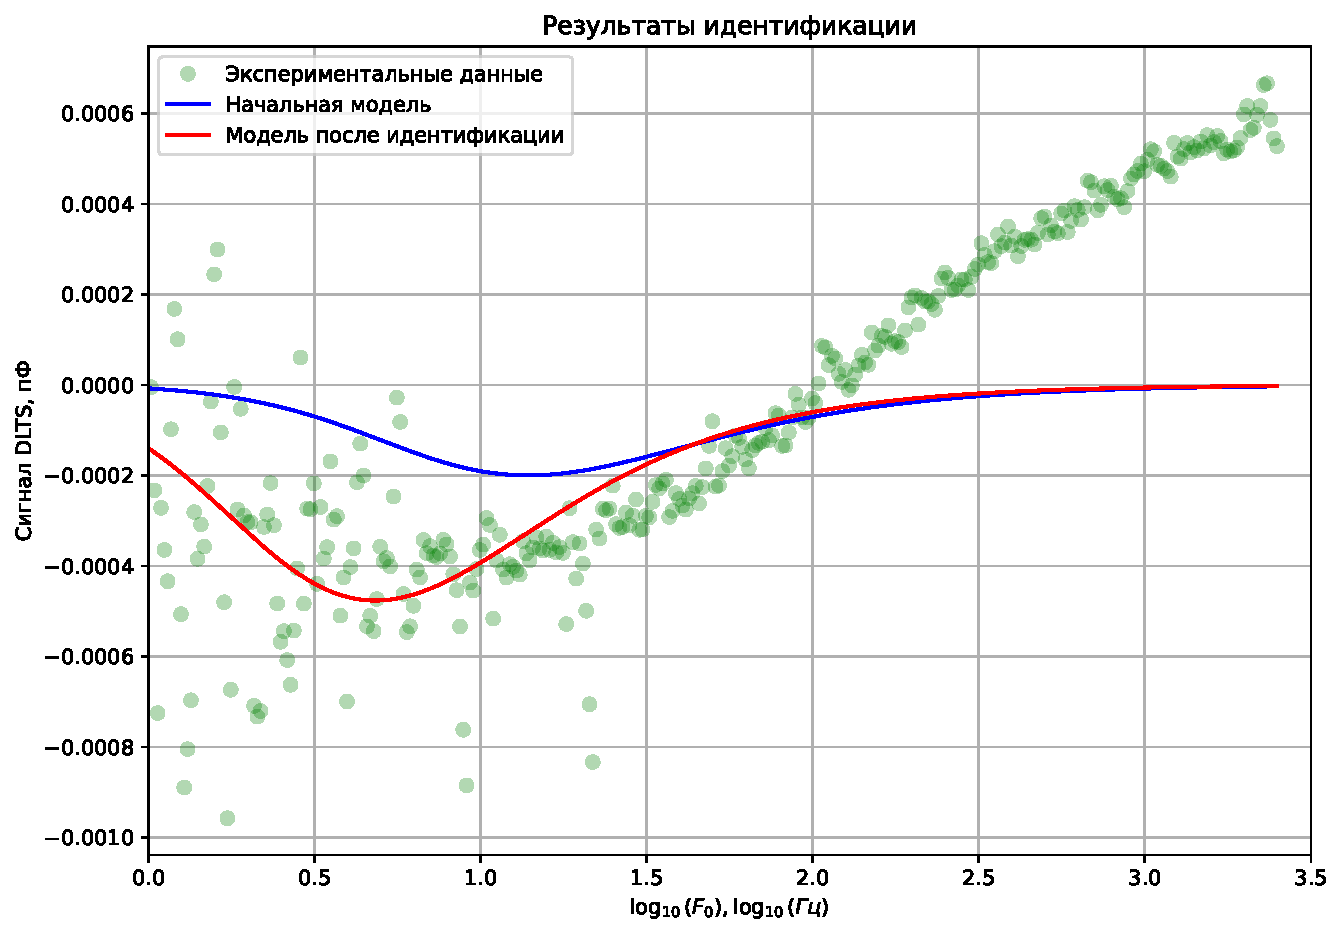
\includegraphics[width=0.75\textwidth]{1564ЛЕ1№1_п1_2500Гц-1Гц_1пФ_-10С_-4В-5В_10мВ_10мкс_шаг_0,01_single_exp_model_2}
		\caption{Результат идентификации отрицательного пика частотного скана
		         при $T=263K$.}
		\label{pic:model_monoexp_p_negative_263}
	\end{figure}

	На рисунке \ref{pic:loss_monoexp_p_negative_263} представлен график значений
	нормированной среднеквадратической ошибки на каждой итерации. На итерациях
	с номерами выше 200 значения среднеквадратической ошибки практически не 
	изменяются, очевидно, алгоритм нашёл минимум.

	\begin{figure}[!htp]
		\centering
		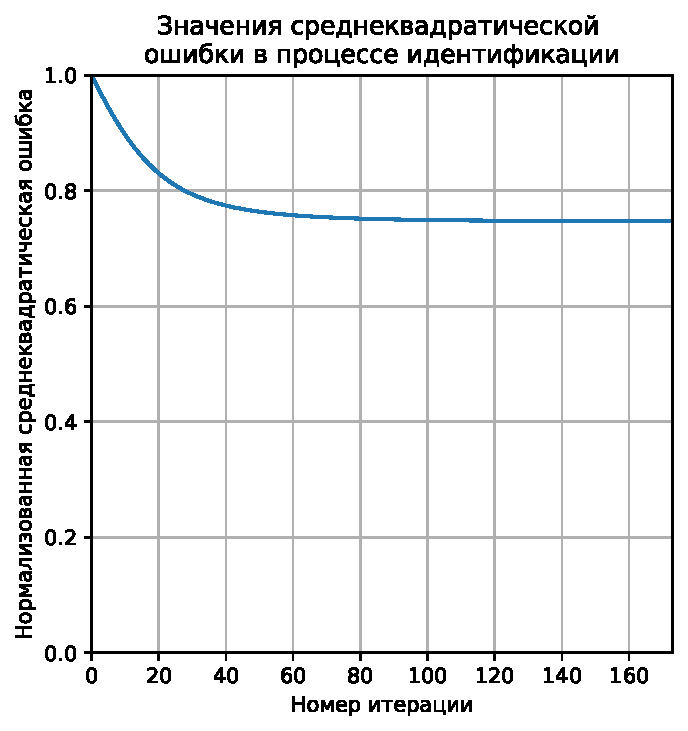
\includegraphics[width=0.35\textwidth]{1564ЛЕ1№1_п1_2500Гц-1Гц_1пФ_-10С_-4В-5В_10мВ_10мкс_шаг_0,01_single_exp_model_loss_2}
		\caption{График среднеквадратической ошибки в процессе идентификации,
		         нормированной относительно её максимального значения.}
		\label{pic:loss_monoexp_p_negative_263}
	\end{figure}

	На гафике отклонений результатов моделирования от экспериментальных данных
	(рисунок \ref{pic:deviations_monoexp_p_negative_263}) видно, что теперь 
	модель <<не охватывает>> диапазон высоких частот опорной функции, где
	располагается положительный пик.

	\begin{figure}[!htp]
		\centering
		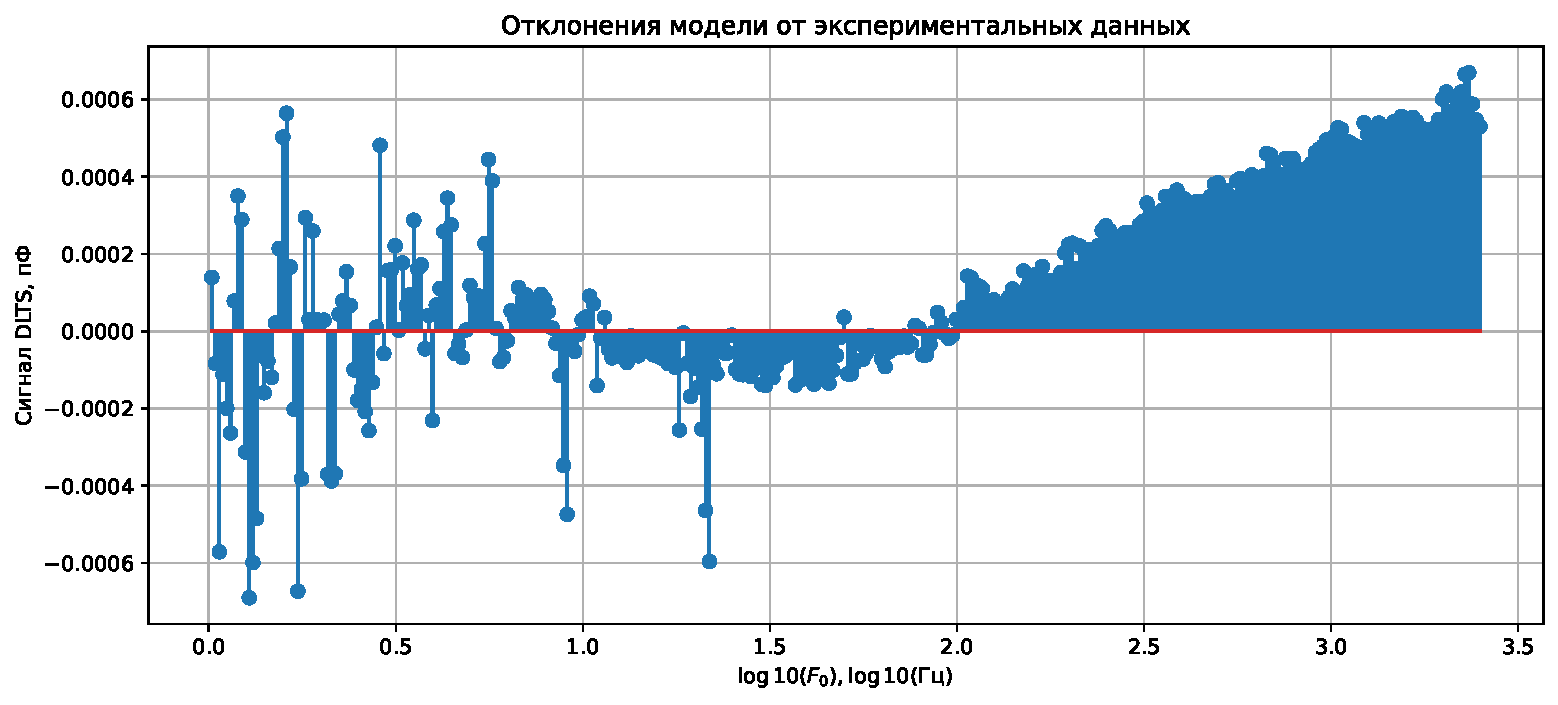
\includegraphics[width=0.75\textwidth]{1564ЛЕ1№1_п1_2500Гц-1Гц_1пФ_-10С_-4В-5В_10мВ_10мкс_шаг_0,01_single_exp_deviations_2}
		\caption{График отклонений результатов, полученных на идентифицированной
		модели, от экспериментальных данных.}
		\label{pic:deviations_monoexp_p_negative_263}
	\end{figure}

	Гистограмма отклонений (рисунок \ref{pic:hist_monoexp_p_negative_263}) 
	далека от нормального распределения. Сплошной линией показан результат 
	сглаживания гистограммы.

	\begin{figure}[!htp]
		\centering
		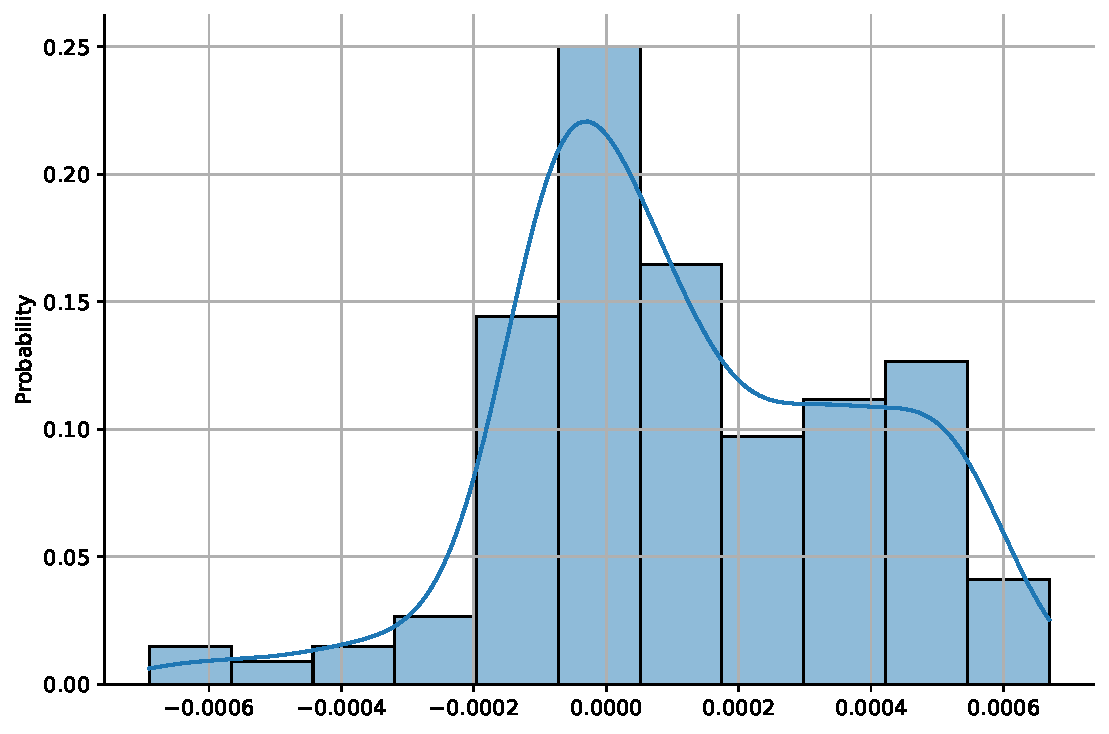
\includegraphics[width=0.5\textwidth]{1564ЛЕ1№1_п1_2500Гц-1Гц_1пФ_-10С_-4В-5В_10мВ_10мкс_шаг_0,01_single_exp_hist_2}
		\caption{Гистограмма отклонений данных, полученных на идентифицированной 
		         модели, от экспериментальных данных. Сплошной линией показан 
		         результат сглаживания гистограммы.}
		\label{pic:hist_monoexp_p_negative_263}
	\end{figure}

	В таблице \ref{table:results_monoexp_p_negative_263} приведём параметры 
	идентифицированной модели и результаты оценок точности моделирования.

	\begin{table}[!htp]
    	\centering
    	\caption{Результаты идентификации модели}
		\begin{tabular}{|l|l|}
			\hline
			Параметр                           & Значение   \\ \hline
			Постоянна времени $\tau$, с        &  0.091434  \\ \hline
			Амплитуда, пФ                      & -0.000476	\\ \hline
			Показатель $p$                     &  1.036     \\ \hline
			Результат кросвалидации (RMSE), пФ &  0.000287  \\ \hline
			RMSE, пФ                           &  0.000286  \\ \hline
		\end{tabular}
		\label{table:results_monoexp_p_negative_263}
	\end{table}

	Построим полученный спектр частотного скана (рисунок 
	\ref{pic:spectr_monoexp_p_negative_263}), чтобы представить результаты в 
	более наглядной форме.

	\begin{figure}[!htp]
		\centering
		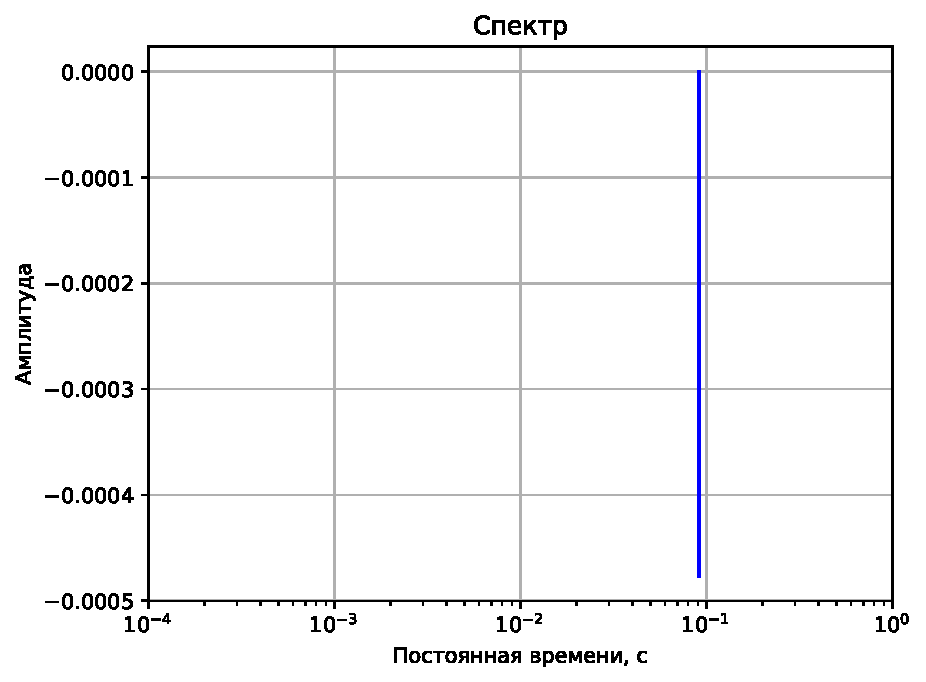
\includegraphics[width=0.5\textwidth]{1564ЛЕ1№1_п1_2500Гц-1Гц_1пФ_-10С_-4В-5В_10мВ_10мкс_шаг_0,01_single_exp_spectr_2}
		\caption{Спектр сигнала релаксации ёмкости.}
		\label{pic:spectr_monoexp_p_negative_263}
	\end{figure}

	
	\newpage
	\subsubsection{Моноэкспоненциальная модель с показателем $p=1$}
	Для сравнения, на тех же данных выполним идентификацию модели идеального 
	частотного скана. В этот раз инициализацию модели выполним случайными 
	значениями. Результаты идентификации представлены на рисунке 
	\ref{pic:model_single_exp_ideal_263}.

	\begin{figure}[!htp]
		\centering
		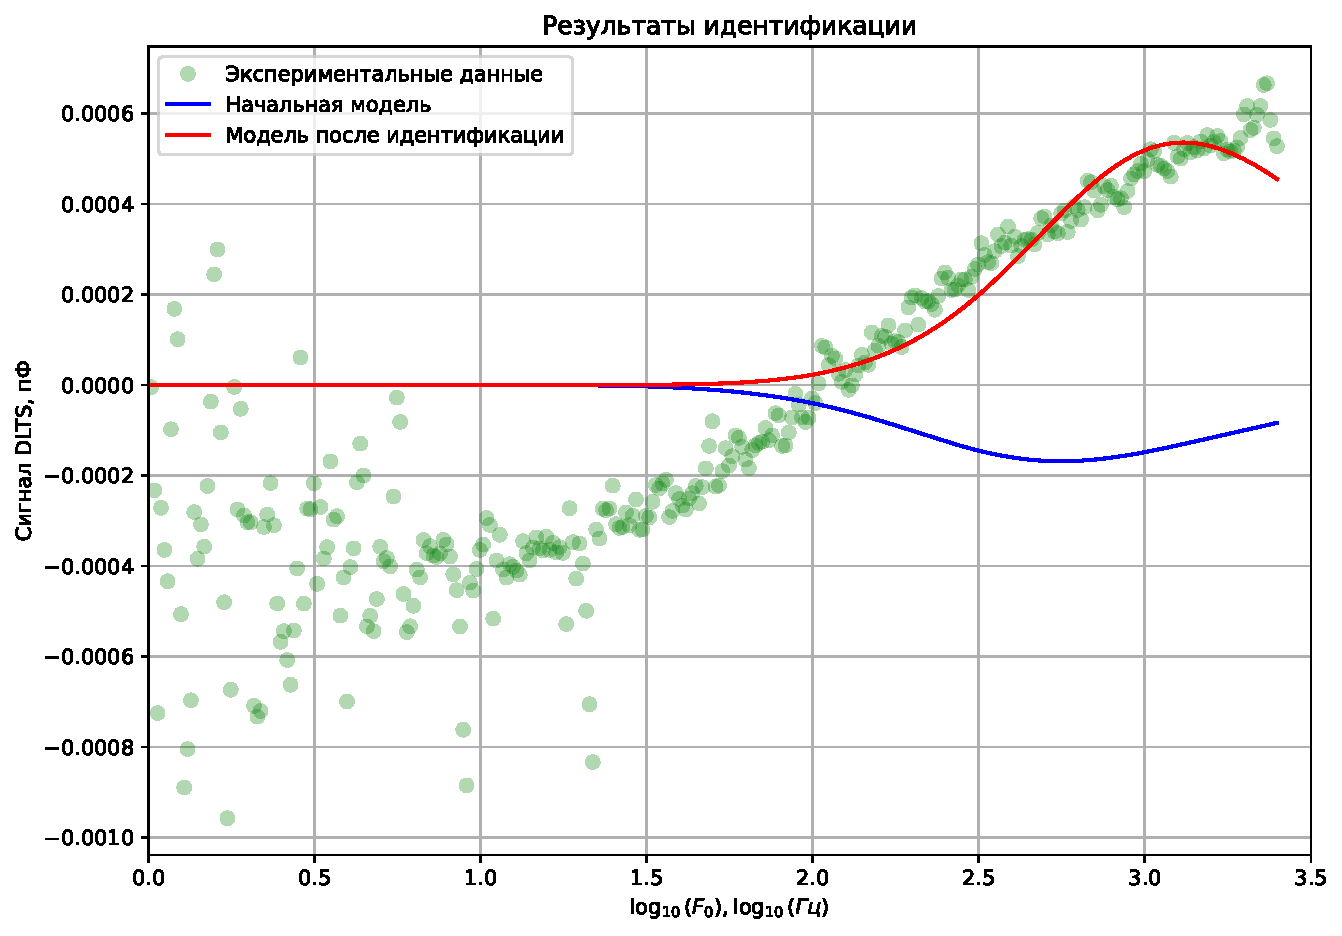
\includegraphics[width=0.75\textwidth]{1564ЛЕ1№1_п1_2500Гц-1Гц_1пФ_-10С_-4В-5В_10мВ_10мкс_шаг_0,01_single_exp_ideal_model}
		\caption{Результат идентификации модели частотного скана при $T=263K$.}
		\label{pic:model_single_exp_ideal_263}
	\end{figure}

	В данном случае алгоритм идентификации нашёл локальный минимум, 
	соответствующий положительному пику. Полученные результаты качественно похожи
	на результаты идентификации из предыдущего раздела. На рисунках 
	\ref{pic:loss_single_exp_ideal_263}, \ref{pic:deviations_single_exp_ideal_263},
	\ref{pic:hist_single_exp_ideal_263} показаны график значений 
	среднеквадратической ошибки на каждой итерации, график отклонений результатов
	моделирования от экспериментальных данных и гистограмма отклонений соответственно.

	\begin{figure}[!htp]
		\centering
		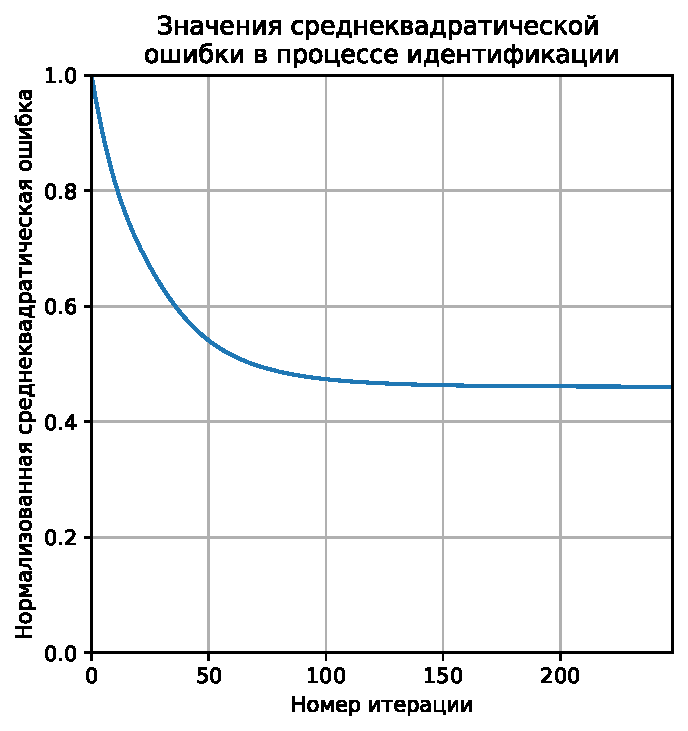
\includegraphics[width=0.35\textwidth]{1564ЛЕ1№1_п1_2500Гц-1Гц_1пФ_-10С_-4В-5В_10мВ_10мкс_шаг_0,01_single_exp_ideal_model_loss}
		\caption{График среднеквадратической ошибки в процессе идентификации,
		         нормированной относительно её максимального значения.}
		\label{pic:loss_single_exp_ideal_263}
	\end{figure}

	\begin{figure}[!htp]
		\centering
		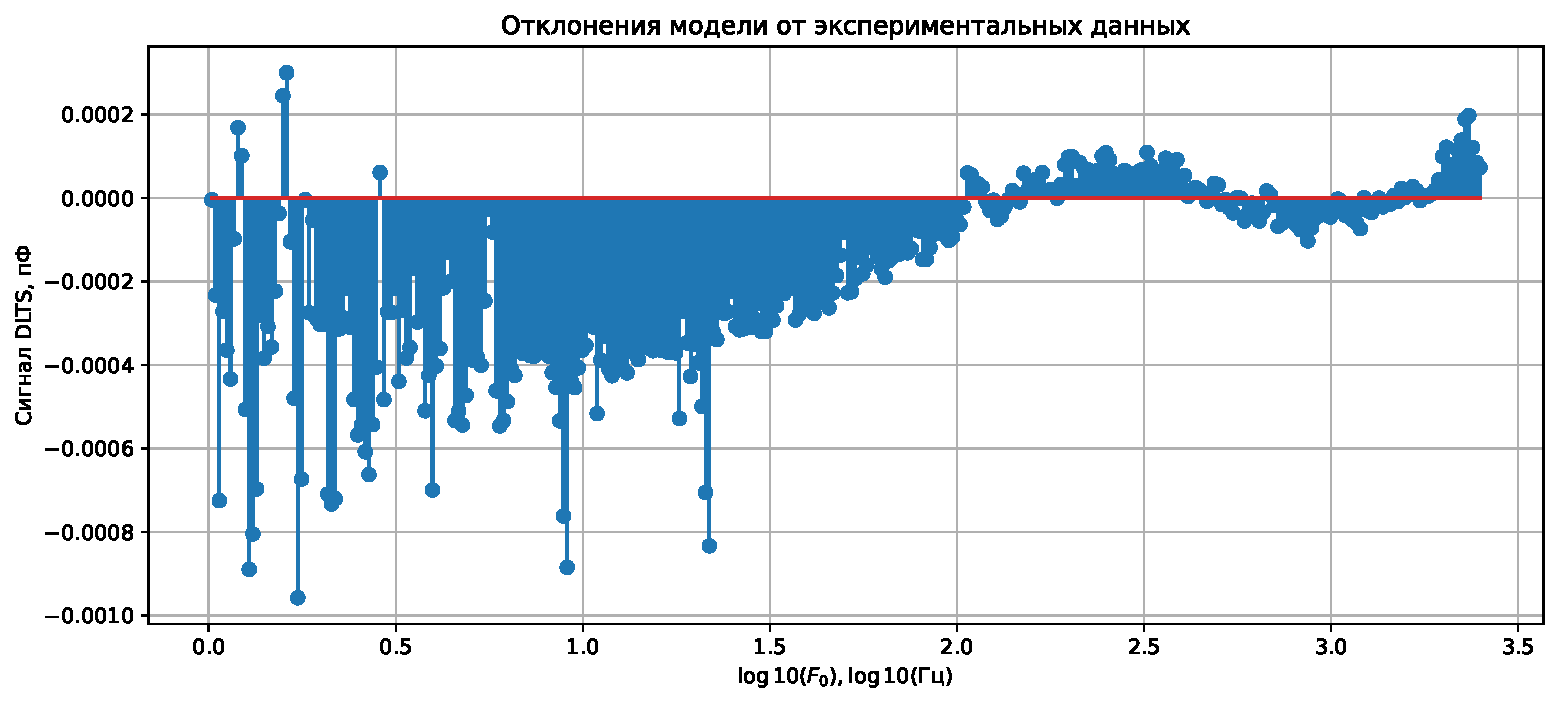
\includegraphics[width=0.75\textwidth]{1564ЛЕ1№1_п1_2500Гц-1Гц_1пФ_-10С_-4В-5В_10мВ_10мкс_шаг_0,01_single_exp_ideal_deviations}
		\caption{График отклонений результатов, полученных на идентифицированной
		модели, от экспериментальных данных.}
		\label{pic:deviations_single_exp_ideal_263}
	\end{figure}

	\begin{figure}[!htp]
		\centering
		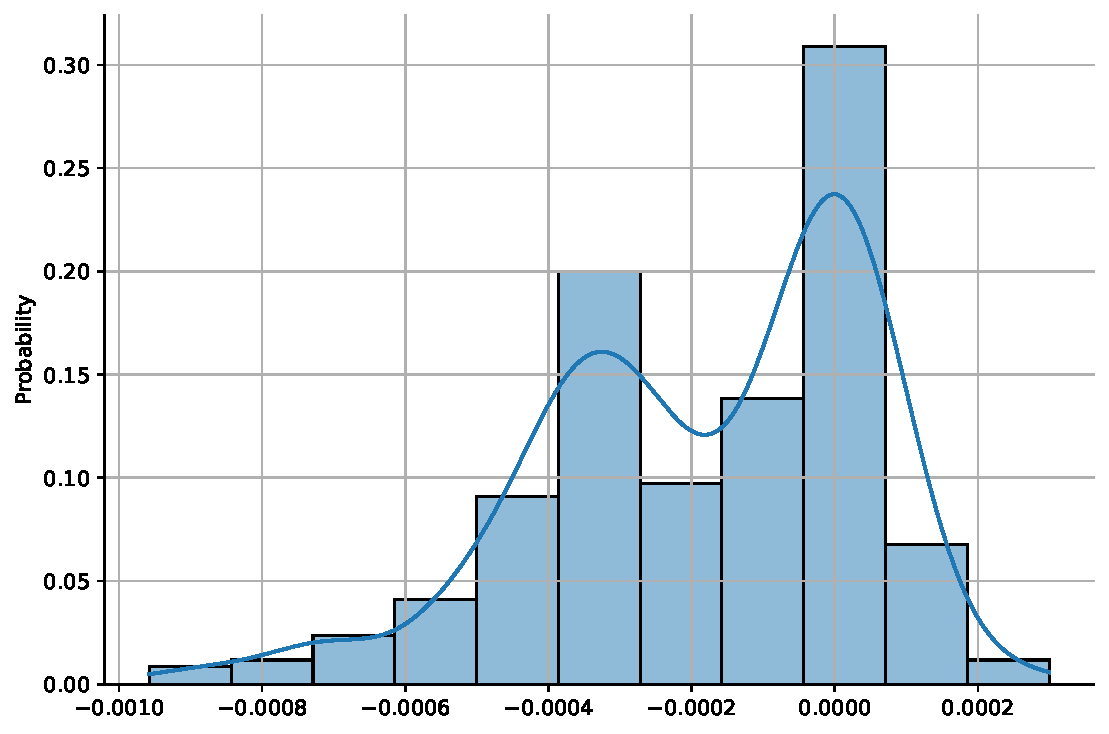
\includegraphics[width=0.5\textwidth]{1564ЛЕ1№1_п1_2500Гц-1Гц_1пФ_-10С_-4В-5В_10мВ_10мкс_шаг_0,01_single_exp_ideal_hist}
		\caption{Гистограмма отклонений данных, полученных на идентифицированной 
		         модели, от экспериментальных данных. Сплошной линией показан 
		         результат сглаживания гистограммы.}
		\label{pic:hist_single_exp_ideal_263}
	\end{figure}

	В таблице \ref{table:results_single_exp_ideal_263} приведены параметры 
	идентифицированной модели и результаты оценок точности моделирования.

	\begin{table}[!htp]
    	\centering
    	\caption{Результаты идентификации модели}
		\begin{tabular}{|l|l|}
			\hline
			Параметр                           & Значение \\ \hline
			Постоянна времени $\tau$, с        & 0.000327 \\ \hline
			Амплитуда, пФ                      & 0.000536 \\ \hline
			Показатель $p$                     & 1.0      \\ \hline
			Результат кросвалидации (RMSE), пФ & 0.000279 \\ \hline
			RMSE, пФ                           & 0.000291 \\ \hline
		\end{tabular}
		\label{table:results_single_exp_ideal_263}
	\end{table}

	На рисунке \ref{pic:spectr_single_exp_ideal_263} приведён полученный спектр 
	частотного скана.

	\begin{figure}[!htp]
		\centering
		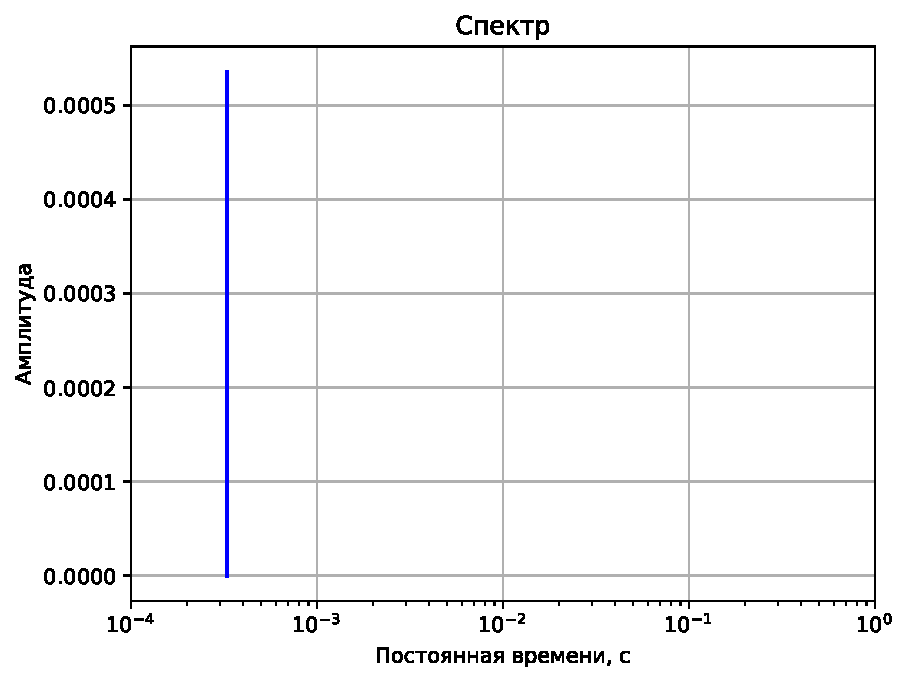
\includegraphics[width=0.5\textwidth]{1564ЛЕ1№1_п1_2500Гц-1Гц_1пФ_-10С_-4В-5В_10мВ_10мкс_шаг_0,01_single_exp_ideal_spectr}
		\caption{Спектр сигнала релаксации ёмкости.}
		\label{pic:spectr_single_exp_ideal_263}
	\end{figure}


	\newpage
	\subsubsection{Многоэкспоненциальная модель с n\_exps > 1}

	Выполним идентификацию многоэкспоненциальной модели. Особенность данной модели
	в том, что у неё есть параметр, независящий от данных -- количество
	экспоененциальных составляющих. По скольку у нас нет гипотезы о количестве
	экспоненциальных составляющих в релаксационном сигнале, воспользуемся приёмом,
	описанном в разделе \ref{section:quality_and_optimization}: для моделей
	с значениями параметра n\_exps равными 5, 6, 7, 8, 9 и 10 будем выполнять
	кросвалидацию, выберем ту, которая покажет лучший результат. В таблице
	\ref{table:multi_exp_model_263_cross_val} предсталены полученные результаты.
	Лучшей оказалась модель с параметром n\_exps = 8, то есть имеющая 8 
	экспоненциальных составляющих.

	\begin{table}[!htp]
    	\centering
    	\caption{Результаты кросвалидации для разных значений параметра n\_exps}
		\begin{tabular}{|l|l|}
		\hline
		Значение параметра n\_exps & Результат кросвалидации \\ \hline
		5                          & 0.0001373               \\ \hline
		6                          & 0.0001361               \\ \hline
		7                          & 0.0001347               \\ \hline
		8                          & 0.0001345               \\ \hline
		9                          & 0.0001353               \\ \hline
		10                         & 0.0001349               \\ \hline
		\end{tabular}
		\label{table:multi_exp_model_263_cross_val}
	\end{table}

	Результаты идентификации модели с восемью экспоненциальными составляющими
	предствалены на рисунке \ref{pic:multi_exp_model_263}. В данном случае,
	модель воспроизводит как положительный так и отрицательный пик.

	\begin{figure}[!htp]
		\centering
		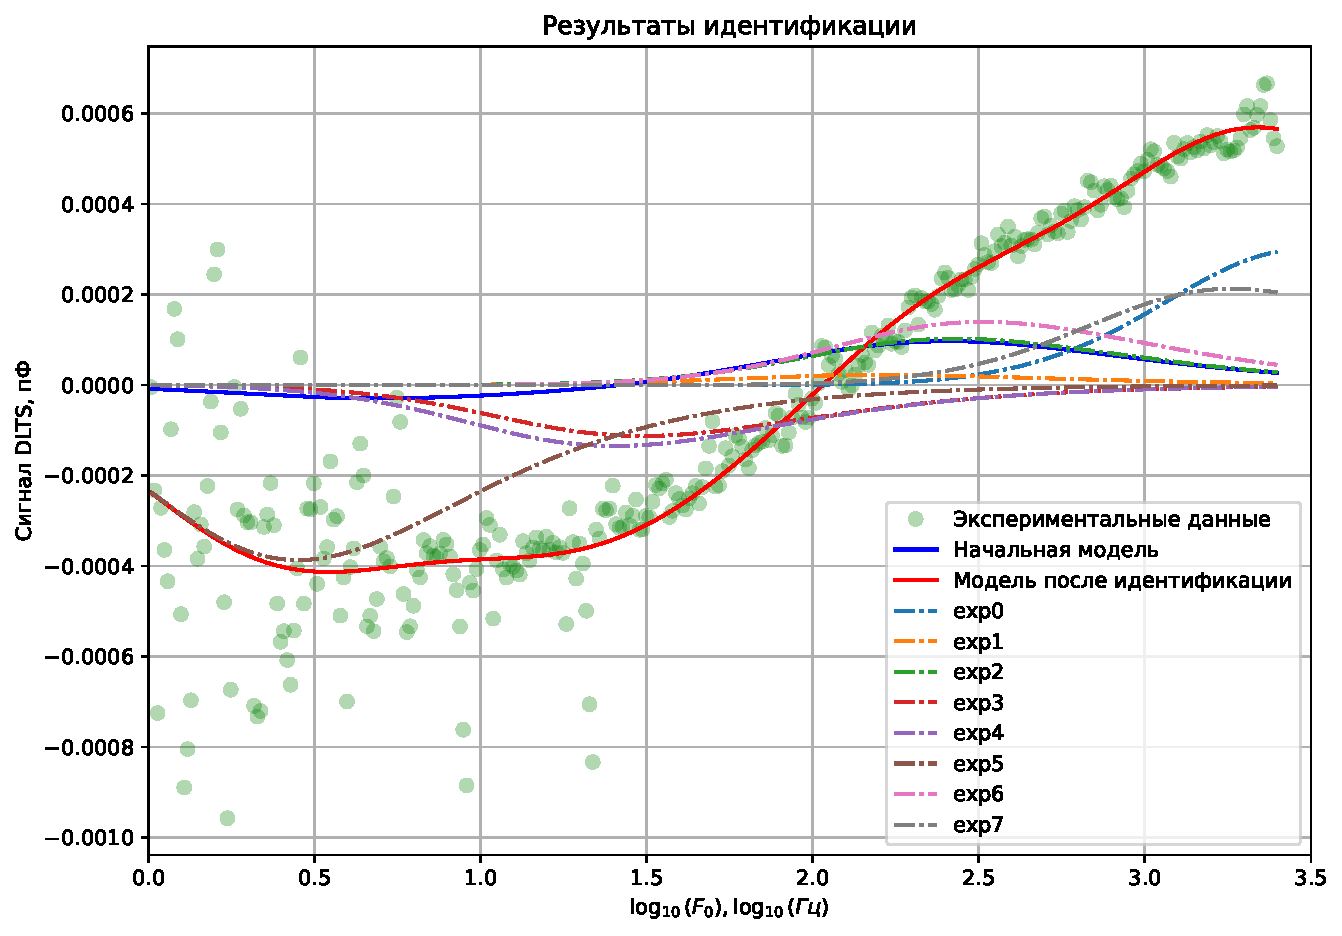
\includegraphics[width=0.75\textwidth]{1564ЛЕ1№1_п1_2500Гц-1Гц_1пФ_-10С_-4В-5В_10мВ_10мкс_шаг_0,01_multi_exp_model}
		\caption{Результат идентификации многоэкспоненциальной моделью 
		         частотного скана при $T=263K$.}
		\label{pic:multi_exp_model_263}
	\end{figure}

	По графику нормированной среднеквадратической ошибки, показанном на рисунке
	\ref{pic:multi_exp_loss_263}, видно, что алгоритм идентификации остановился
	из-за достижения максимального количества итераций. При этом, форма графика
	позволяет предположить, что полученные параметры модели близки к оптимальным.

	\begin{figure}[!htp]
		\centering
		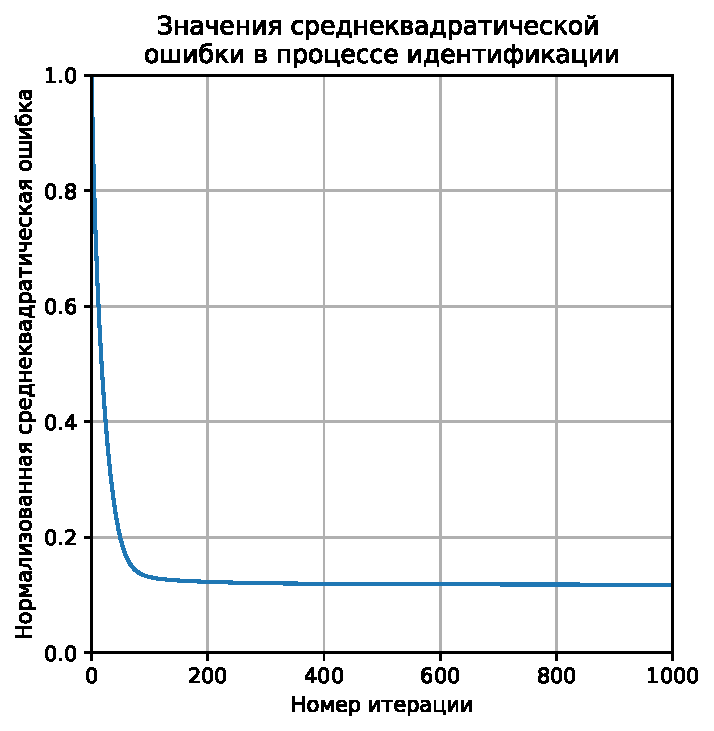
\includegraphics[width=0.35\textwidth]{1564ЛЕ1№1_п1_2500Гц-1Гц_1пФ_-10С_-4В-5В_10мВ_10мкс_шаг_0,01_multi_exp_loss}
		\caption{График среднеквадратической ошибки в процессе идентификации,
		         нормированной относительно её максимального значения.}
		\label{pic:multi_exp_loss_263}
	\end{figure}

	На рисунке \ref{pic:multi_exp_deviations_263} показан график отклонений
	результатов моделирования от экспериментальных данных. В отличие от двух
	предыдущих моделей, многоэкспоненциальная модель хорошо воспроизводит 
	как положительный, так и отрицательный пик. Увеличение разброса в области
	низких частот опорной функции связано с особенностями работы аппаратного
	интегратора спектрометра.

	\begin{figure}[!htp]
		\centering
		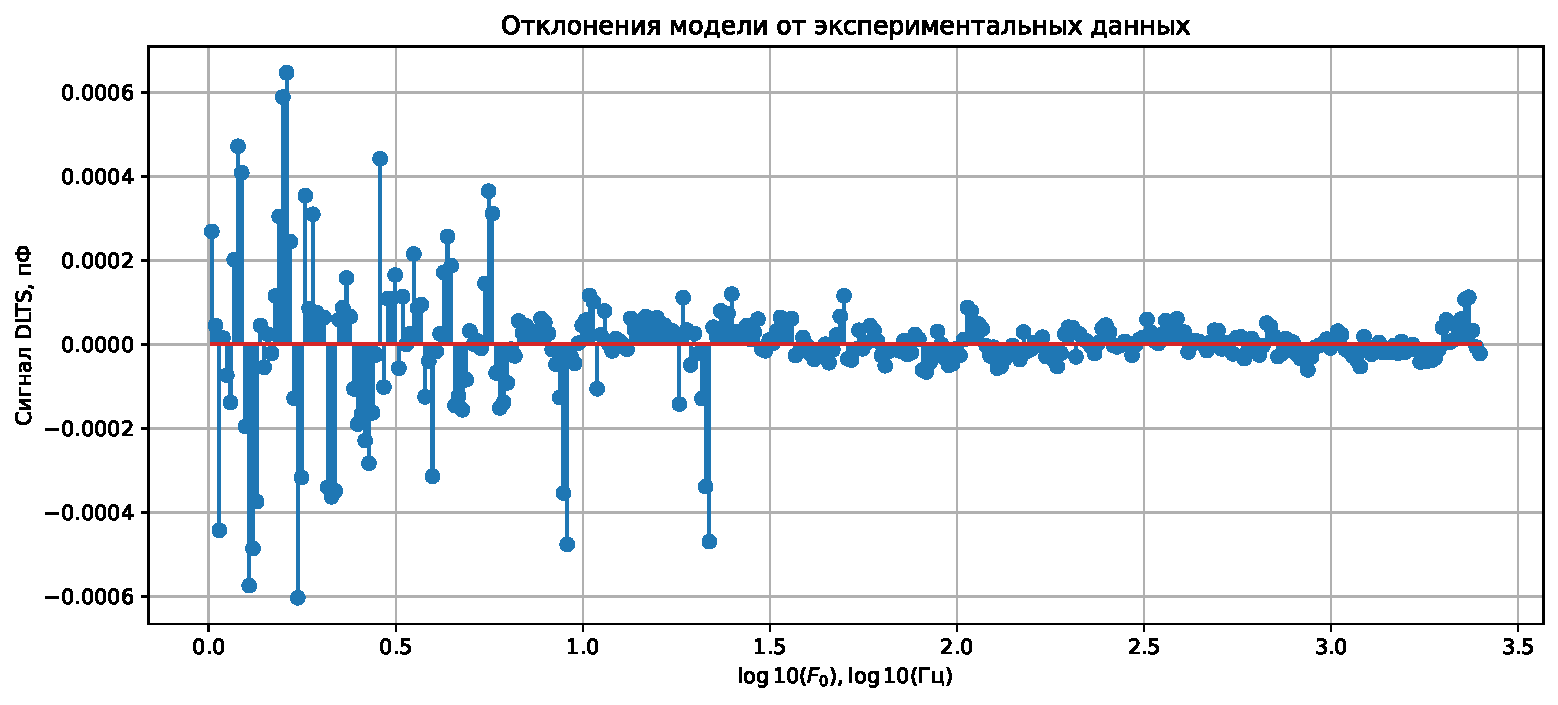
\includegraphics[width=0.75\textwidth]{1564ЛЕ1№1_п1_2500Гц-1Гц_1пФ_-10С_-4В-5В_10мВ_10мкс_шаг_0,01_multi_exp_deviations}
		\caption{График отклонений результатов, полученных на идентифицированной
		модели, от экспериментальных данных.}
		\label{pic:multi_exp_deviations_263}
	\end{figure}

	На рисунке \ref{pic:multi_exp_hist_263} показана гистограмма отклонений 
	данных, полученных на идентифицированной модели, от результатов измерений.
	Форма полученного распределения приближается к форме нормального распределения.

	\begin{figure}[!htp]
		\centering
		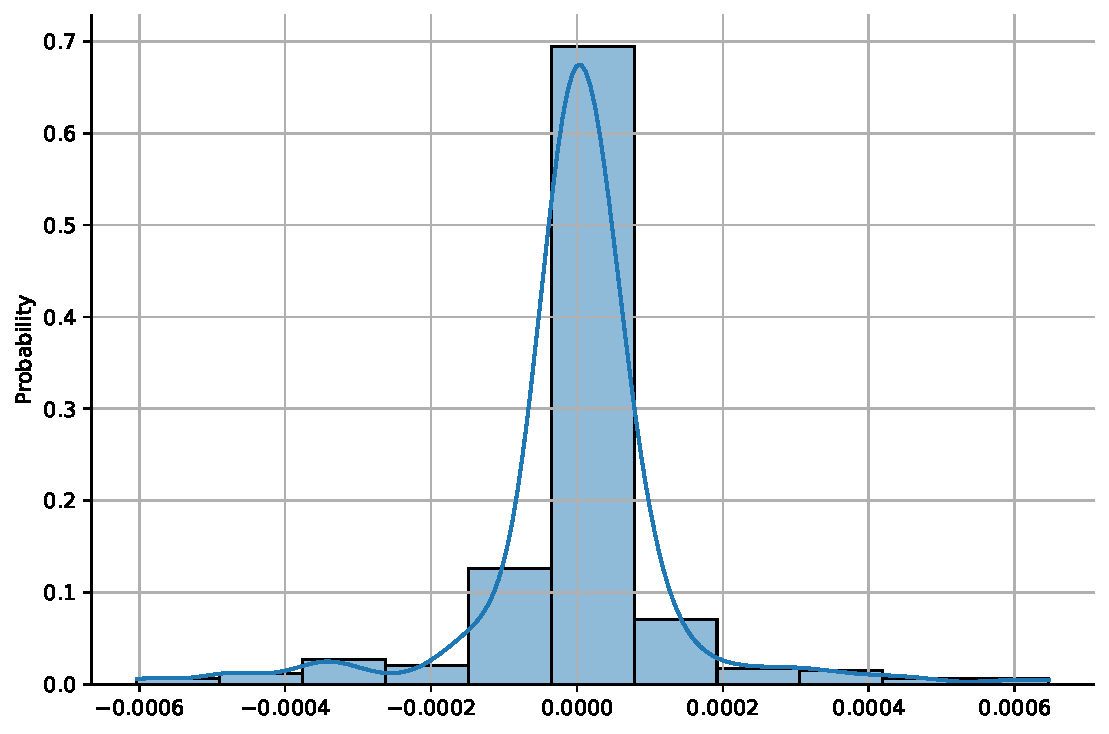
\includegraphics[width=0.5\textwidth]{1564ЛЕ1№1_п1_2500Гц-1Гц_1пФ_-10С_-4В-5В_10мВ_10мкс_шаг_0,01_multi_exp_hist}
		\caption{Гистограмма отклонений данных, полученных на идентифицированной 
		         модели, от экспериментальных данных. Сплошной линией показан 
		         результат сглаживания гистограммы.}
		\label{pic:multi_exp_hist_263}
	\end{figure}

	В таблице \ref{table:multi_exp_results_263} приведены параметры 
	идентифицированной модели и результаты оценок точности моделирования,  
	$\tau$ -- постоянная времени, $A$ -- амплитуда.

	\begin{table}[!htp]
    	\centering
    	\caption{Результаты идентификации модели.}
		\begin{tabular}{|l|l|l|l|}
			\hline
			Параметр                           & Значение & Параметр  & Значение  \\ \hline
			$\tau_1$, с                        & 0.000132 & $A_1$, пФ &  0.000301 \\ \hline
			$\tau_2$, с                        & 0.002744 & $A_2$, пФ &  0.000022 \\ \hline
			$\tau_3$, с                        & 0.001629 & $A_3$, пФ &  0.000102 \\ \hline
			$\tau_4$, с                        & 0.014347 & $A_4$, пФ & -0.000113 \\ \hline
			$\tau_5$, с                        & 0.017352 & $A_5$, пФ & -0.000135 \\ \hline
			$\tau_6$, с                        & 0.156241 & $A_6$, пФ & -0.000387 \\ \hline
			$\tau_7$, с                        & 0.001342 & $A_7$, пФ &  0.000139 \\ \hline
			$\tau_8$, с                        & 0.000230 & $A_8$, пФ &  0.000213 \\ \hline
			Результат кросвалидации (RMSE), пФ & 0.000134 &           &           \\ \hline
			RMSE, пФ                           & 0.000132 &           &           \\ \hline
		\end{tabular}
		\label{table:multi_exp_results_263}
	\end{table}

	На рисунке \ref{pic:multi_exp_spectr_263} приведён полученный спектр 
	частотного скана.

	\begin{figure}[!htp]
		\centering
		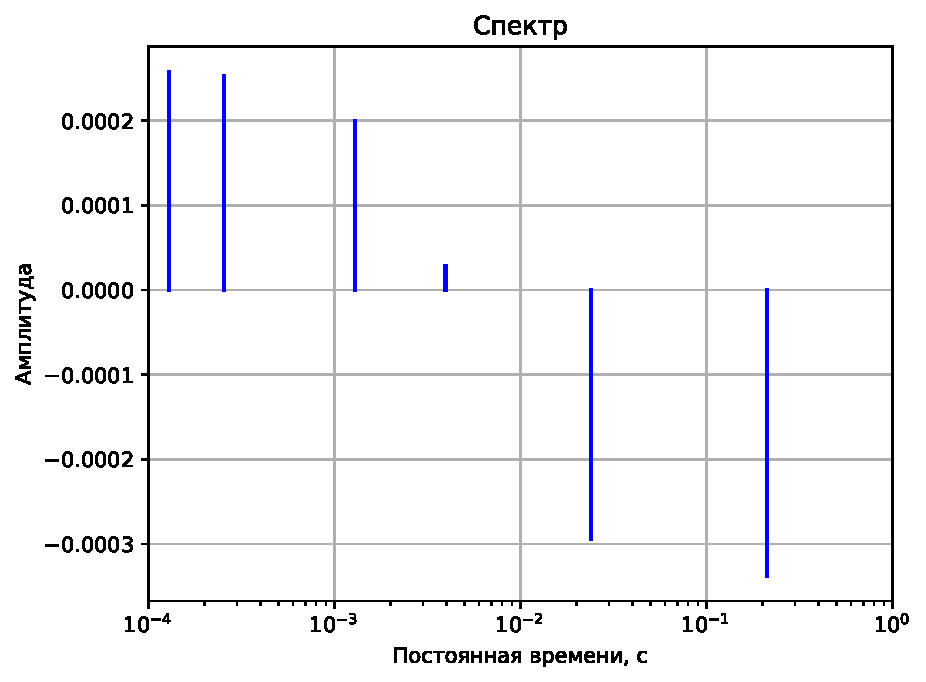
\includegraphics[width=0.5\textwidth]{1564ЛЕ1№1_п1_2500Гц-1Гц_1пФ_-10С_-4В-5В_10мВ_10мкс_шаг_0,01_multi_exp_spectr}
		\caption{Спектр сигнала релаксации ёмкости.}
		\label{pic:multi_exp_spectr_263}
	\end{figure}


	\newpage
	\subsubsection{Сравнение результатов}
	В таблице \ref{table:model_comparison_263} представлено сравнение результатов
	оценки точности рассмотренных моделей. В то время как модель идеального
	частотного скана (положительный пик) и модели c показателем $p$ показывают 
	приблизительно одинаковые результаты, многоэкспоненциальная модель показывает
	вдвое более высокую точность.
	
	\begin{table}[!htp]
	\centering
	\caption{Результаты идентификации моделей.}
	\begin{tabular}{|l|l|l|}
		\hline
		Модель                    & Результат         & RMSE, пФ \\ 
		                          & кросвалидации, пФ &          \\ \hline
		Идеаьный частотный скан   & 0.000279          & 0.000291 \\ \hline
		Модель с показателем $p$  & 0.000290          & 0.000291 \\
		(положительный пик)       &                   &          \\ \hline
		Модель с показателем $p$  & 0.000287          & 0.000286 \\ 
		(отрицательный пик)       &                   &          \\ \hline
		Многоэкспоененциальная    & 0.000134          & 0.000132 \\
		модель                    &                   &          \\ \hline
	\end{tabular}
	\label{table:model_comparison_263}
	\end{table}



	\newpage
	\subsection{Частотный скан при температуре 283 К}
	\subsubsection{Моноэкспоненциальная модель с показателем $p$}
	Результаты измерений при температуре 283~К приведены на рисунке 
	\ref{pic:train_data_283}. Полученный частотный скан имеет один пик,
	положительной полярности. Результаты идентификации модели с показателем 
	$p$ приведены на рисунке \ref{pic:single_exp_model_283}.

	\begin{figure}[!htp]
		\centering
		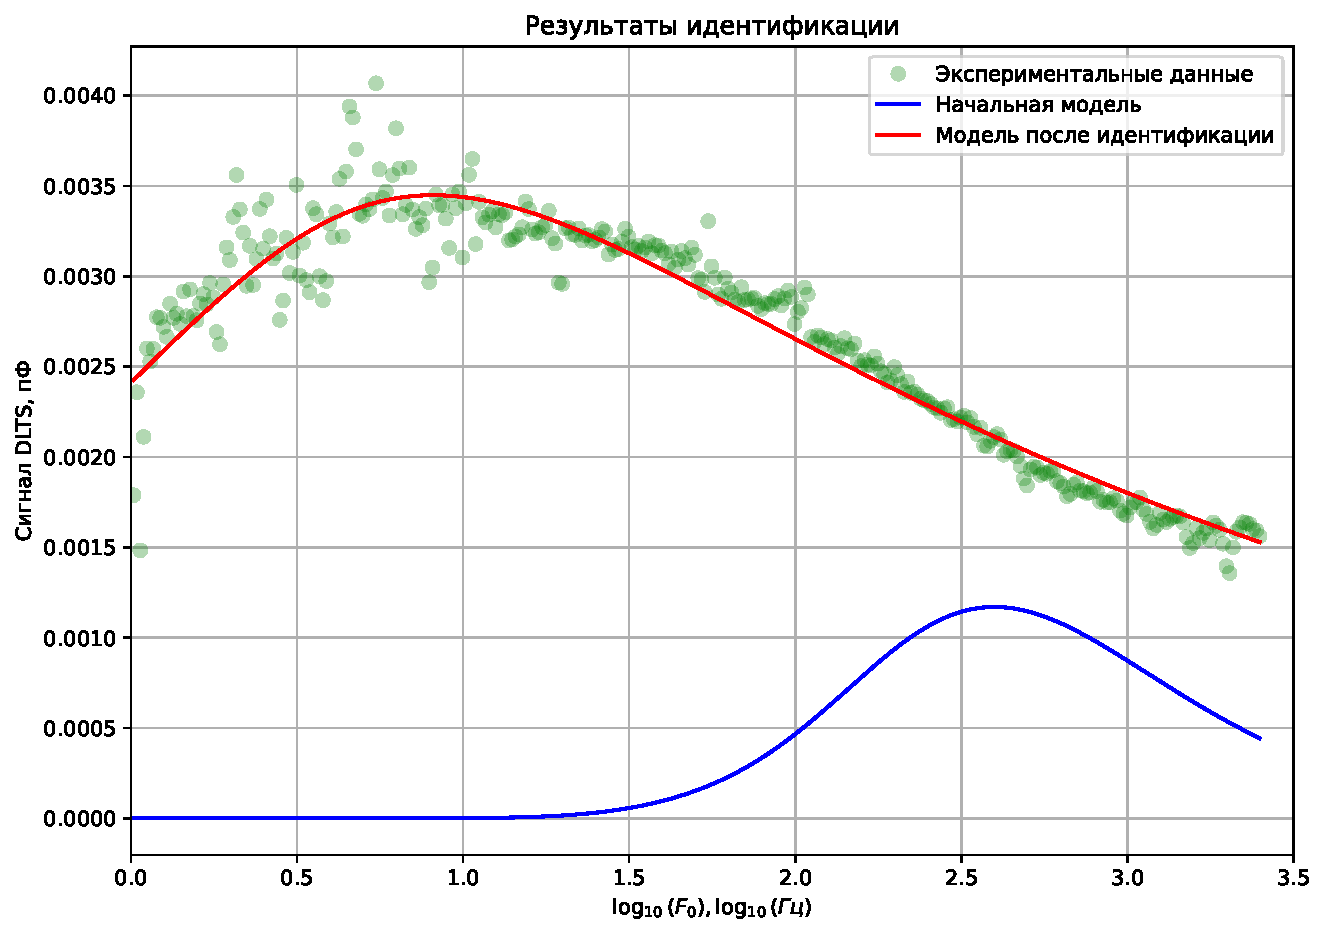
\includegraphics[width=0.75\textwidth]{1564ЛЕ1№1_п1_2500Гц-1Гц_1пФ_+10С_-4В-5В_50мВ_10мкс_шаг_0,01_single_exp_model}
		\caption{Результат идентификации частотного скана при $T=283K$.}
		\label{pic:single_exp_model_283}
	\end{figure}

	График нормированной среднеквадратической ошибки подтверждает на рисунке
	\ref{pic:loss_single_exp_283}, что алгоритм идентификации нашёл минимум 
	функции потерь.

	\begin{figure}[!htp]
		\centering
		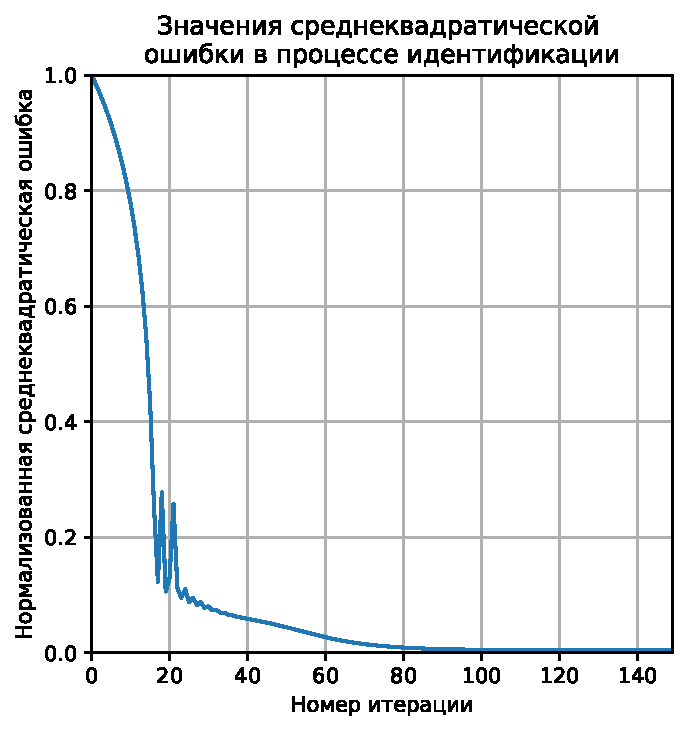
\includegraphics[width=0.35\textwidth]{1564ЛЕ1№1_п1_2500Гц-1Гц_1пФ_+10С_-4В-5В_50мВ_10мкс_шаг_0,01_single_exp_model_loss}
		\caption{График среднеквадратической ошибки в процессе идентификации,
		         нормированной относительно её максимального значения.}
		\label{pic:loss_single_exp_283}
	\end{figure}

	На рисунках \ref{pic:deviations_single_exp_283} и \ref{pic:hist_single_exp_283}
	показаны график отклонений результатов моделирования от экспериментальных
	данных и гистограмма отклонений. Гистограмма по форме близка к нормальному
	закону.

	\begin{figure}[!htp]
		\centering
		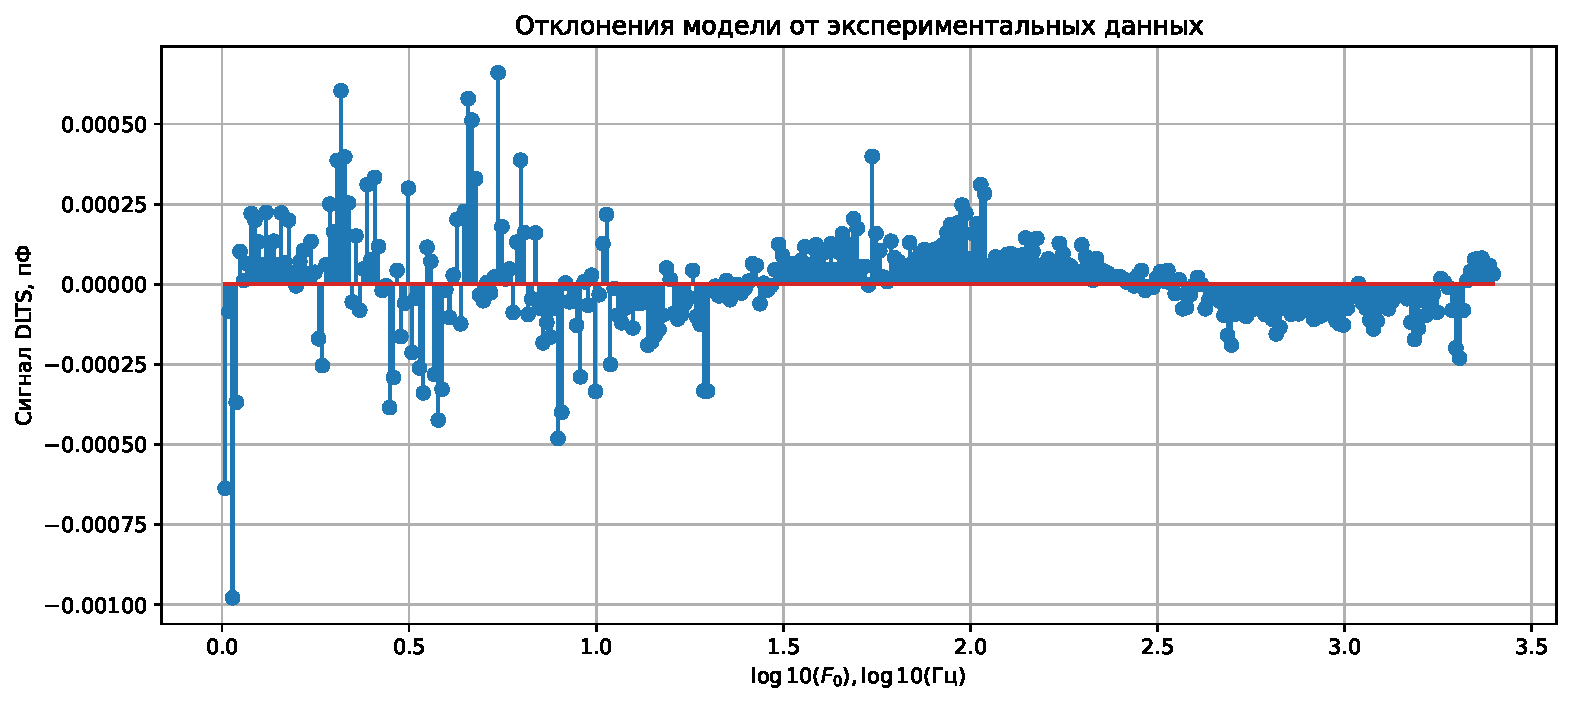
\includegraphics[width=0.75\textwidth]{1564ЛЕ1№1_п1_2500Гц-1Гц_1пФ_+10С_-4В-5В_50мВ_10мкс_шаг_0,01_single_exp_deviations}
		\caption{График отклонений результатов, полученных на идентифицированной
		модели, от экспериментальных данных.}
		\label{pic:deviations_single_exp_283}
	\end{figure}

	\begin{figure}[!htp]
		\centering
		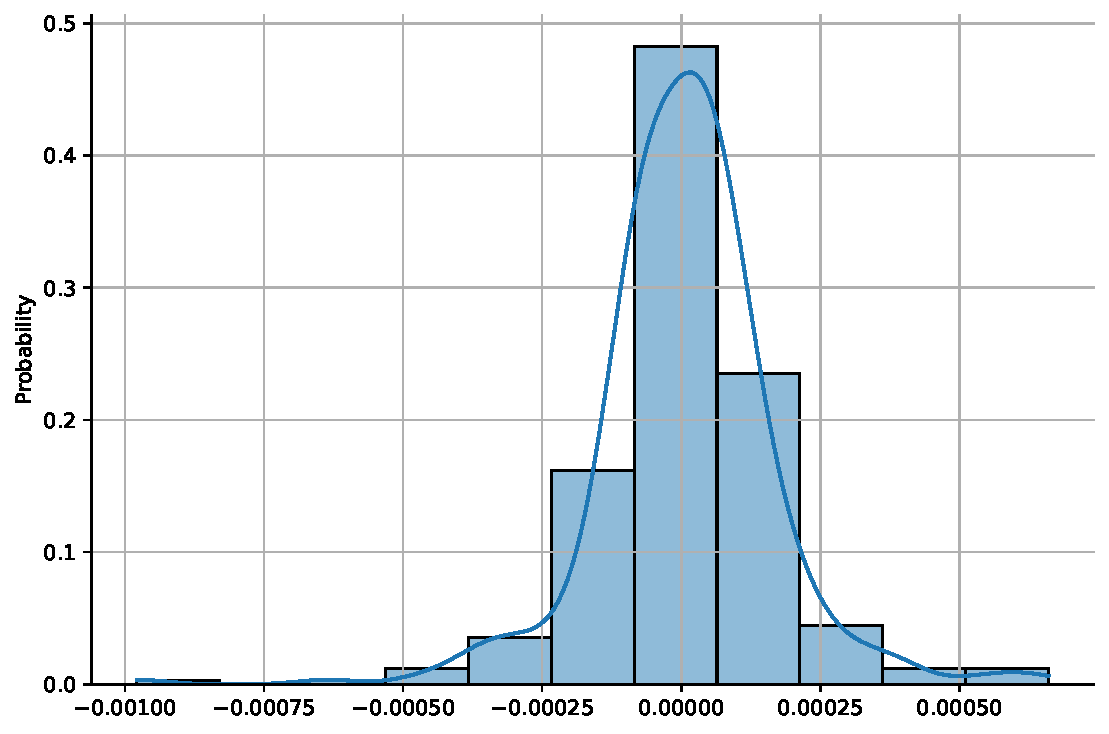
\includegraphics[width=0.5\textwidth]{1564ЛЕ1№1_п1_2500Гц-1Гц_1пФ_+10С_-4В-5В_50мВ_10мкс_шаг_0,01_single_exp_hist}
		\caption{Гистограмма отклонений данных, полученных на идентифицированной 
		         модели, от экспериментальных данных. Сплошной линией показан
		         результат сглаживания гистограммы.}
		\label{pic:hist_single_exp_283}
	\end{figure}

	В таблице \ref{table:results_single_exp_283} приведены параметры 
	идентифицированной модели и результаты оценок точности моделирования.

	\begin{table}[!htp]
		\centering
		\caption{Результаты идентификации модели}
		\begin{tabular}{|l|l|}
			\hline
			Параметр                           & Значение \\ \hline
			Постоянна времени $\tau$, с        & 0,054291 \\ \hline
			Амплитуда, пФ                      & 0.003448 \\ \hline
			Показатель $p$                     & 0.173    \\ \hline
			Результат кросвалидации (RMSE), пФ & 0.000160 \\ \hline
			RMSE, пФ                           & 0.000161 \\ \hline
		\end{tabular}
		\label{table:results_single_exp_283}
	\end{table}

	На рисунке \ref{pic:multi_exp_spectr_283} приведён полученный спектр 
	частотного скана.

	\begin{figure}[!htp]
		\centering
		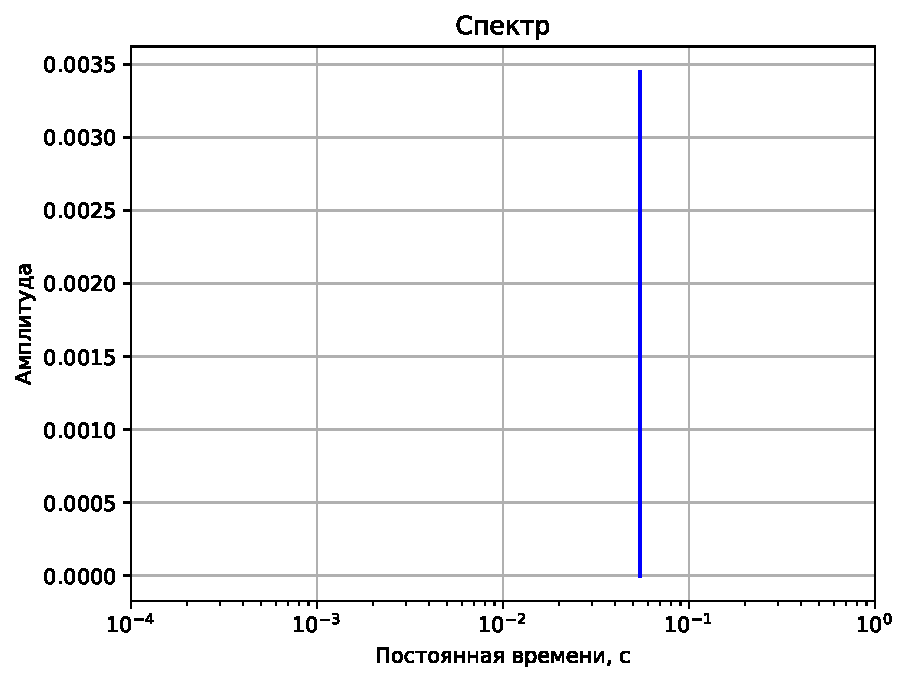
\includegraphics[width=0.5\textwidth]{1564ЛЕ1№1_п1_2500Гц-1Гц_1пФ_+10С_-4В-5В_50мВ_10мкс_шаг_0,01_single_exp_spectr}
		\caption{Спектр сигнала релаксации ёмкости.}
		\label{pic:spectr_single_exp_283}
	\end{figure}


	\newpage
	\subsubsection{Моноэкспоненциальная модель с показателем $p = 1$}

	Выполним идентификацию модели идеального частотного скана на результатах,
	полученных при температуре 283~К. Результаты идентификации модели приведены 
	на рисунке \ref{pic:model_single_exp_ideal_283}. На графике заметны
	существенные отклонения результатов моделирования от экспериментальных 
	данных, при этом, график значений нормированной среднеквадратической ошибки
	для каждой итерации (рисунок \ref{pic:loss_single_exp_ideal_283}) 
	свидетельствует о том, что алгоритм идентификации нашёл минимум функции 
	потерь.

	\begin{figure}[!htp]
		\centering
		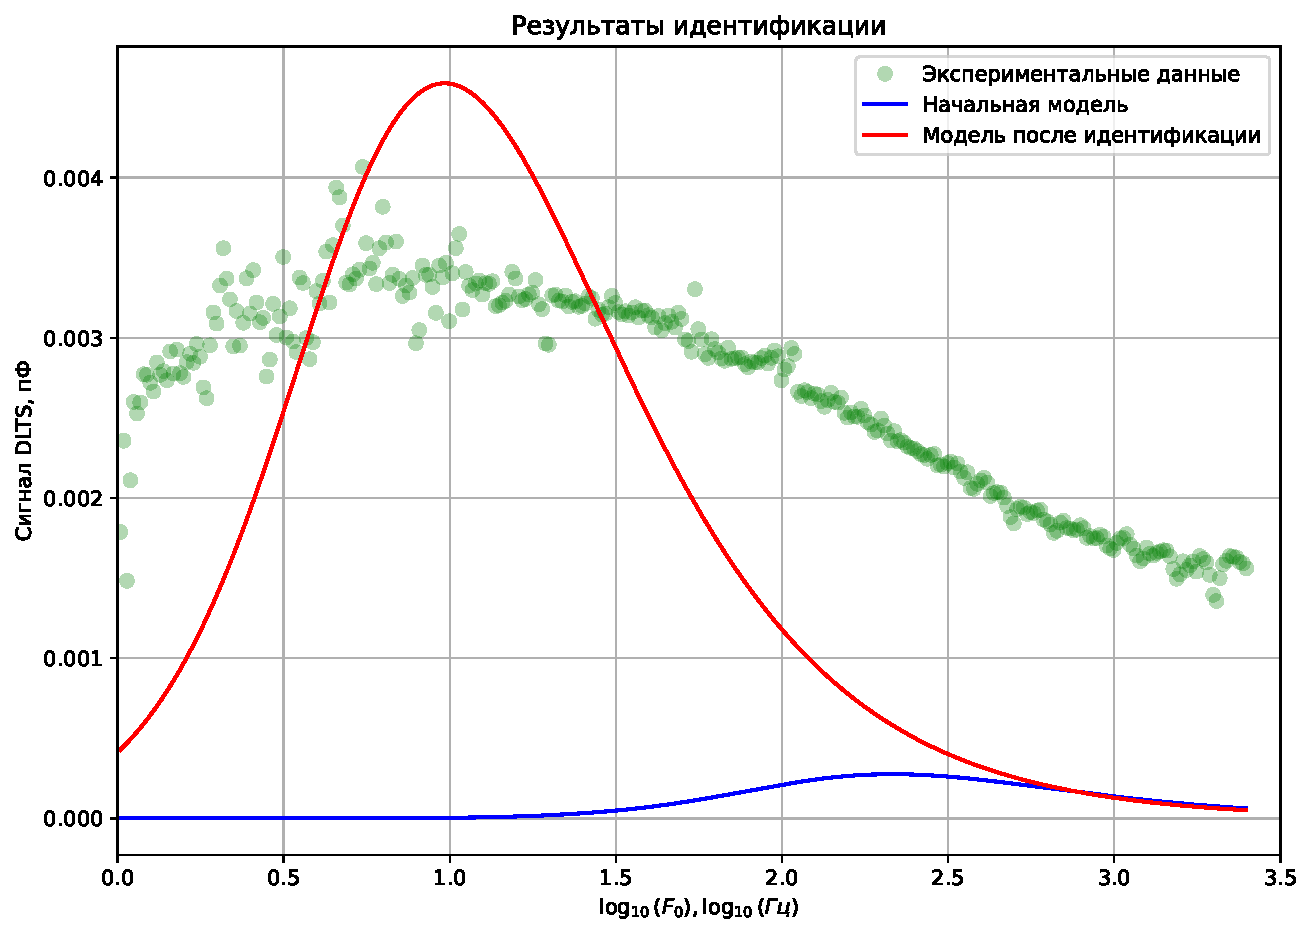
\includegraphics[width=0.75\textwidth]{1564ЛЕ1№1_п1_2500Гц-1Гц_1пФ_+10С_-4В-5В_50мВ_10мкс_шаг_0,01_single_exp_ideal_model}
		\caption{Результат идентификации частотного скана при $T=283K$.}
		\label{pic:model_single_exp_ideal_283}
	\end{figure}

	\begin{figure}[!htp]
		\centering
		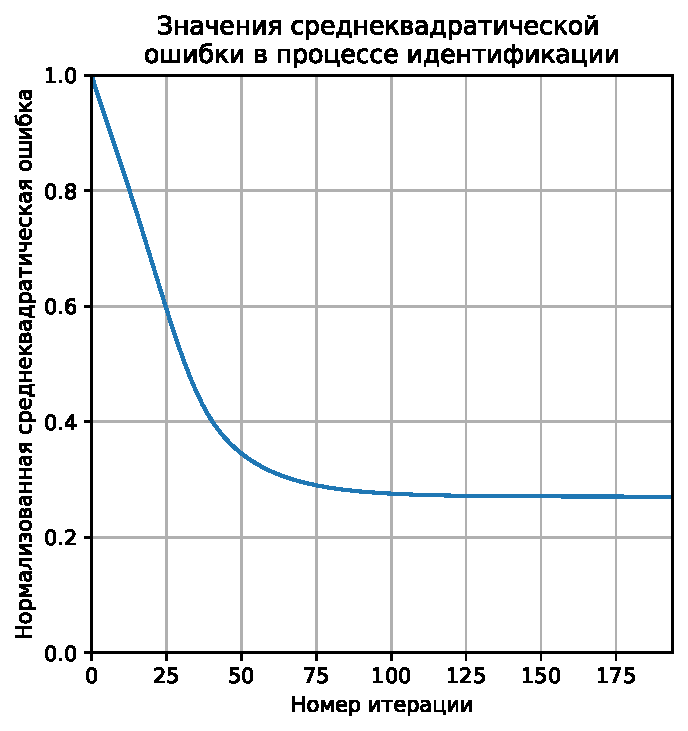
\includegraphics[width=0.35\textwidth]{1564ЛЕ1№1_п1_2500Гц-1Гц_1пФ_+10С_-4В-5В_50мВ_10мкс_шаг_0,01_single_exp_ideal_model_loss}
		\caption{График среднеквадратической ошибки в процессе идентификации,
		         нормированной относительно её максимального значения.}
		\label{pic:loss_single_exp_ideal_283}
	\end{figure}

	График отклонений результатов моделирования от экспериментальных данных 
	(рисунок \ref{pic:deviations_single_exp_ideal_283}) также демонстрирует
	значительные систематические отклонения. Закономерно, гистограмма (рисунок
	\ref{pic:hist_single_exp_ideal_283}) по форме далека от нормального
	распределения.

	\begin{figure}[!htp]
		\centering
		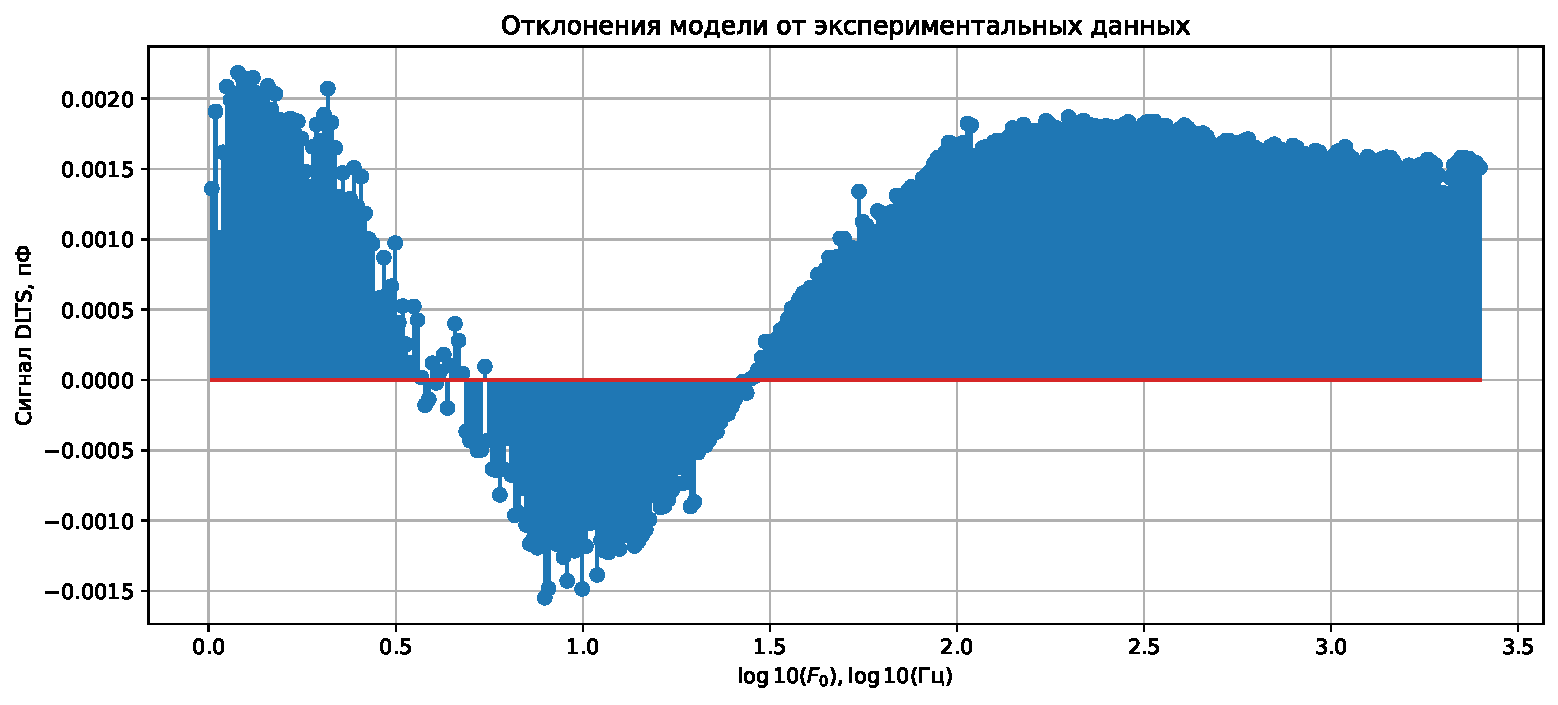
\includegraphics[width=0.75\textwidth]{1564ЛЕ1№1_п1_2500Гц-1Гц_1пФ_+10С_-4В-5В_50мВ_10мкс_шаг_0,01_single_exp_ideal_deviations}
		\caption{График отклонений результатов, полученных на идентифицированной
		модели, от экспериментальных данных.}
		\label{pic:deviations_single_exp_ideal_283}
	\end{figure}

	\begin{figure}[!htp]
		\centering
		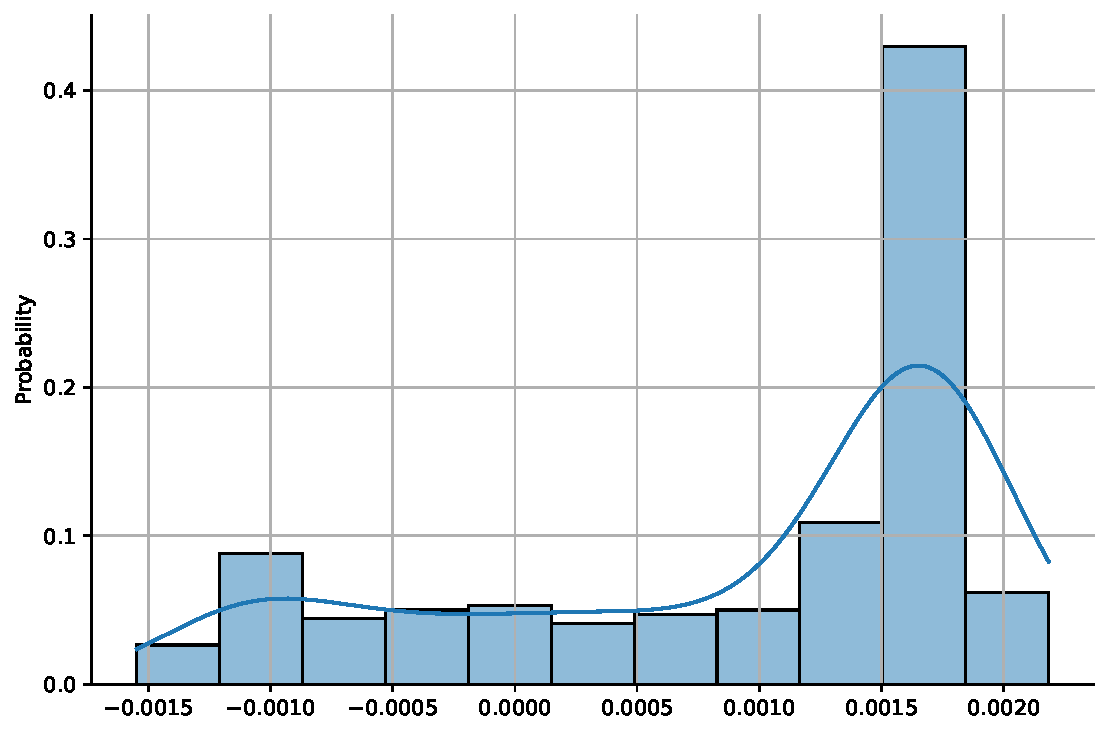
\includegraphics[width=0.5\textwidth]{1564ЛЕ1№1_п1_2500Гц-1Гц_1пФ_+10С_-4В-5В_50мВ_10мкс_шаг_0,01_single_exp_ideal_hist}
		\caption{Гистограмма отклонений данных, полученных на идентифицированной 
		         модели, от экспериментальных данных. Сплошной линией показан
		         результат сглаживания гистограммы.}
		\label{pic:hist_single_exp_ideal_283}
	\end{figure}

	В таблице \ref{table:results_single_exp_ideal_283} приведены параметры 
	идентифицированной модели и результаты оценок точности моделирования.

	\begin{table}[!htp]
		\centering
		\caption{Результаты идентификации модели}
		\begin{tabular}{|l|l|}
			\hline
			Параметр                           & Значение \\ \hline
			Постоянна времени $\tau$, с        & 0.045708 \\ \hline
			Амплитуда, пФ                      & 0.004591 \\ \hline
			Показатель $p$                     & 1.0      \\ \hline
			Результат кросвалидации (RMSE), пФ & 0.001396 \\ \hline
			RMSE, пФ                           & 0.001389 \\ \hline
		\end{tabular}
		\label{table:results_single_exp_ideal_283}
	\end{table}

	На рисунке \ref{pic:spectr_single_exp_ideal_283} приведён полученный спектр 
	частотного скана.

	\begin{figure}[!htp]
		\centering
		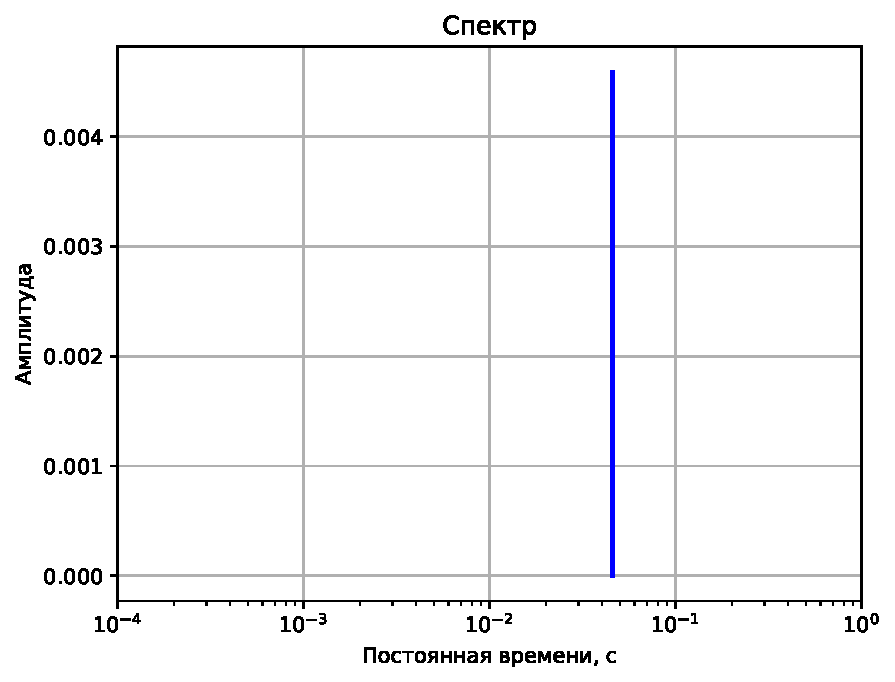
\includegraphics[width=0.5\textwidth]{1564ЛЕ1№1_п1_2500Гц-1Гц_1пФ_+10С_-4В-5В_50мВ_10мкс_шаг_0,01_single_exp_ideal_spectr}
		\caption{Спектр сигнала релаксации ёмкости.}
		\label{pic:spectr_single_exp_ideal_283}
	\end{figure}


	\newpage
	\subsubsection{Многоэкспоненциальная модель с n\_exps > 1}
	Выполним идентификацию многоэкспоненциальной модели, для этого сравним
	результаты кросвалидации для моделей, имеющих значения парамера n\_exps
	равные 5, 6, 7, 8, 9 и 10, и выберем показавшую лучший результат. В таблице
	\ref{table:multi_exp_model_283_cross_val} представлены полученные результаты.
	Лучшей оказалась модель с параметром n\_exps = 6, то есть имеющая 6 
	экспоненциальных составляющих.

	\begin{table}[!htp]
		\centering
		\caption{Результаты кросвалидации для разных значений параметра n\_exps}
		\begin{tabular}{|l|l|}
		\hline
		Значение параметра n\_exps & Результат кросвалидации \\ \hline
		5                          & 0.0001579               \\ \hline
		6                          & 0.0001530               \\ \hline
		7                          & 0.0001532               \\ \hline
		8                          & 0.0001547               \\ \hline
		9                          & 0.0001537               \\ \hline
		10                         & 0.0001546               \\ \hline
		\end{tabular}
		\label{table:multi_exp_model_283_cross_val}
	\end{table}

	Результаты идентификации модели с шестью экспоненциальными составляющими
	представлены на рисунке \ref{pic:multi_exp_model_283}.

	\begin{figure}[!htp]
		\centering
		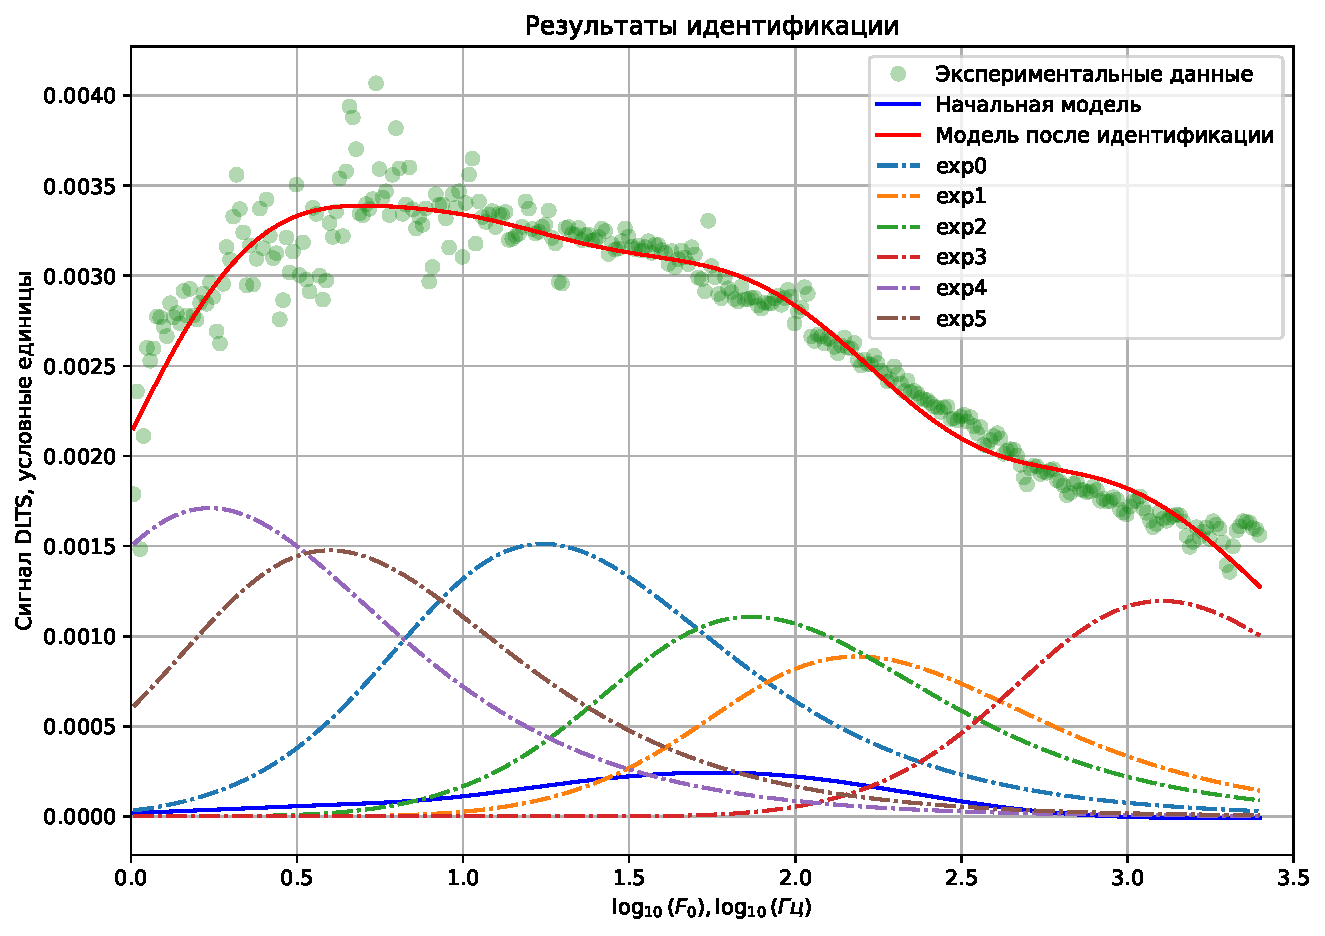
\includegraphics[width=0.75\textwidth]{1564ЛЕ1№1_п1_2500Гц-1Гц_1пФ_+10С_-4В-5В_50мВ_10мкс_шаг_0,01_multi_exp_model}
		\caption{Результат идентификации многоэкспоненциальной моделью 
		         частотного скана при $T=283K$.}
		\label{pic:multi_exp_model_283}
	\end{figure}

	На рисунке \ref{pic:multi_exp_loss_283} показан график нормированной
	среднеквадратической ошибки. Форма графика говорит о том, что алгоритм
	идентификации нашёл минимум функции потерь.

	\begin{figure}[!htp]
		\centering
		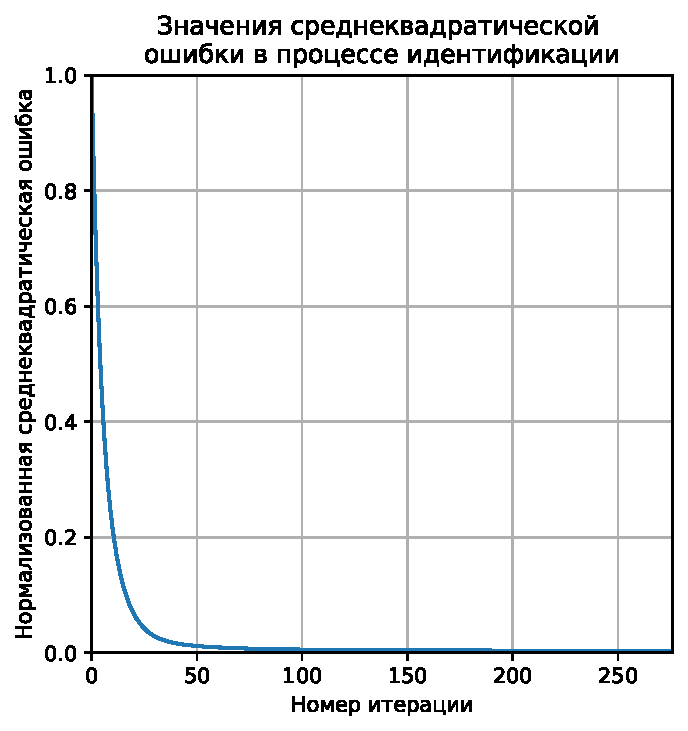
\includegraphics[width=0.35\textwidth]{1564ЛЕ1№1_п1_2500Гц-1Гц_1пФ_+10С_-4В-5В_50мВ_10мкс_шаг_0,01_multi_exp_loss}
		\caption{График среднеквадратической ошибки в процессе идентификации,
		         нормированной относительно её максимального значения.}
		\label{pic:multi_exp_loss_283}
	\end{figure}

	На графике отклонений результатов моделирования от экспериментальных данных
	(рисунок \ref{pic:multi_exp_deviations_283}) заметны систематические отклонения
	в области высоких значенией частоты опорной функции. Они же заметны на 
	рисунке \ref{pic:multi_exp_model_283}. Их появление может быть связано с 
	влиянием случайной инициализации модели -- алгоритм из-за <<неудачных>> 
	начальных значений завершил работу вблизи минимума функции потерь, но
	самого минимума так и не достиг.

	\begin{figure}[!htp]
		\centering
		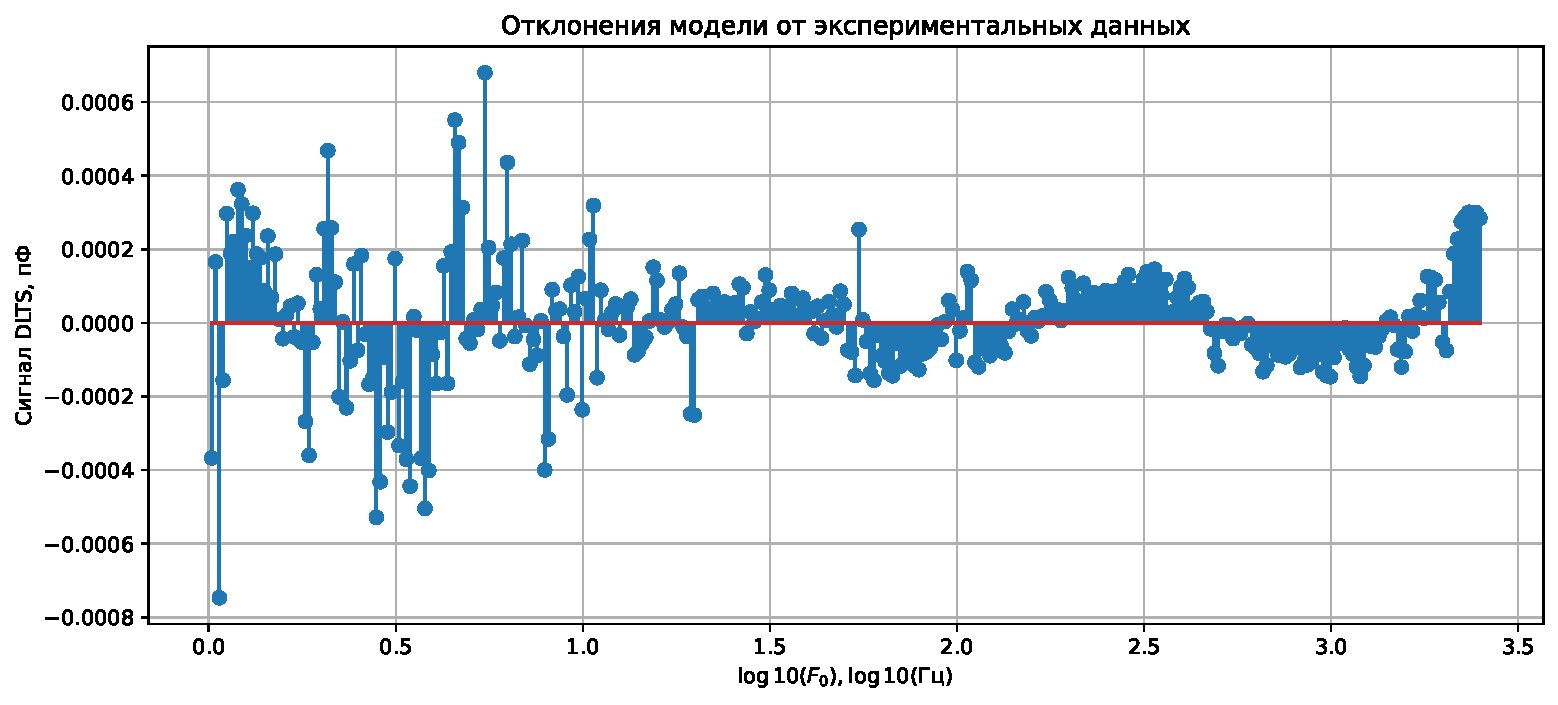
\includegraphics[width=0.75\textwidth]{1564ЛЕ1№1_п1_2500Гц-1Гц_1пФ_+10С_-4В-5В_50мВ_10мкс_шаг_0,01_multi_exp_deviations}
		\caption{График отклонений результатов, полученных на идентифицированной
		модели, от экспериментальных данных.}
		\label{pic:multi_exp_deviations_283}
	\end{figure}

	На рисунке \ref{pic:multi_exp_hist_283} показана гистограмма отклонений 
	результатов моделирования от экспериментальных данных. Форма гистограммы 
	близка к форме нормального распределения.

	\begin{figure}[!htp]
		\centering
		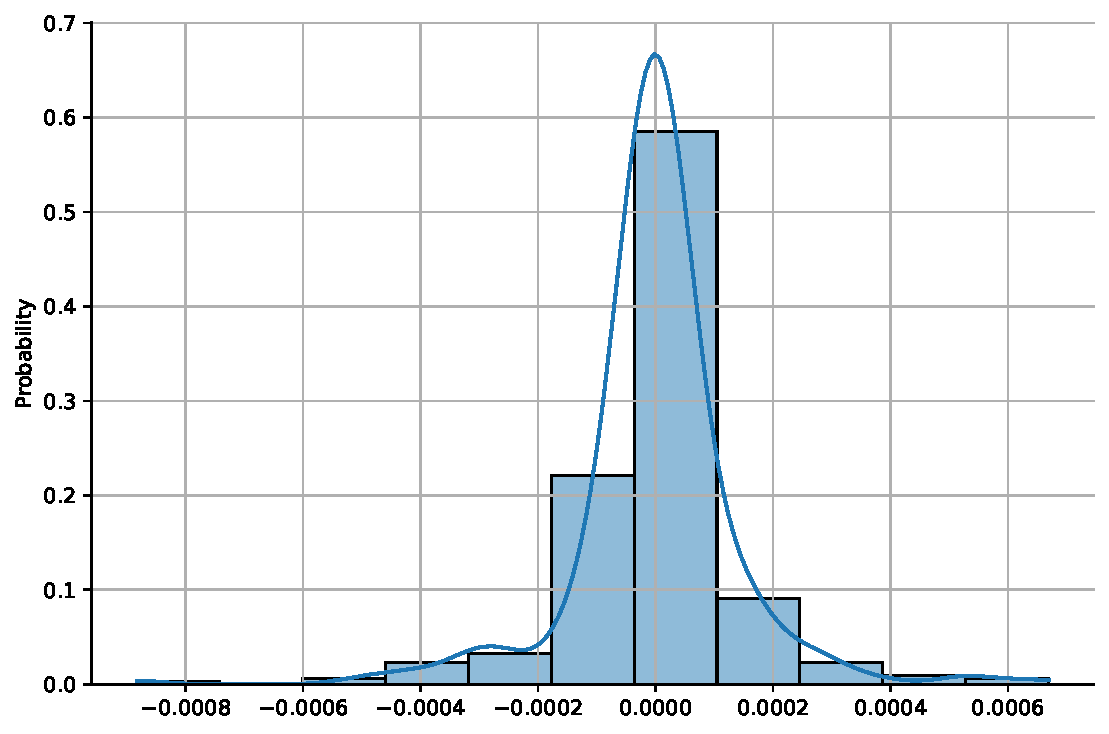
\includegraphics[width=0.5\textwidth]{1564ЛЕ1№1_п1_2500Гц-1Гц_1пФ_+10С_-4В-5В_50мВ_10мкс_шаг_0,01_multi_exp_hist}
		\caption{Гистограмма отклонений данных, полученных на идентифицированной 
		         модели, от экспериментальных данных. Сплошной линией показан
		         результат сглаживания гистограммы.}
		\label{pic:multi_exp_hist_283}
	\end{figure}

	В таблице \ref{table:multi_exp_results_283} приведены параметры 
	идентифицированной модели и результаты оценок точности моделирования,  
	$\tau$ -- постоянная времени, $A$ -- амплитуда.

	\begin{table}[!htp]
		\centering
		\caption{Результаты идентификации модели.}
		\begin{tabular}{|l|l|l|l|}
			\hline
			Параметр                           & Значение & Параметр  & Значение  \\ \hline
			$\tau_1$, с                        & 0.025388 & $A_1$, пФ & 0.001513  \\ \hline
			$\tau_2$, с                        & 0.002868 & $A_2$, пФ & 0.000887  \\ \hline
			$\tau_3$, с                        & 0.005958 & $A_3$, пФ & 0.001108  \\ \hline
			$\tau_4$, с                        & 0.000336 & $A_4$, пФ & 0.001196  \\ \hline
			$\tau_5$, с                        & 0.255645 & $A_5$, пФ & 0.001711  \\ \hline
			$\tau_6$, с                        & 0.111247 & $A_6$, пФ & 0.001476  \\ \hline
			Результат кросвалидации (RMSE), пФ & 0.000158 &           &           \\ \hline
			RMSE, пФ                           & 0.000156 &           &           \\ \hline
		\end{tabular}
		\label{table:multi_exp_results_283}
	\end{table}

	На рисунке \ref{pic:multi_exp_spectr_283} приведён полученный спектр 
	частотного скана.

	\begin{figure}[!htp]
		\centering
		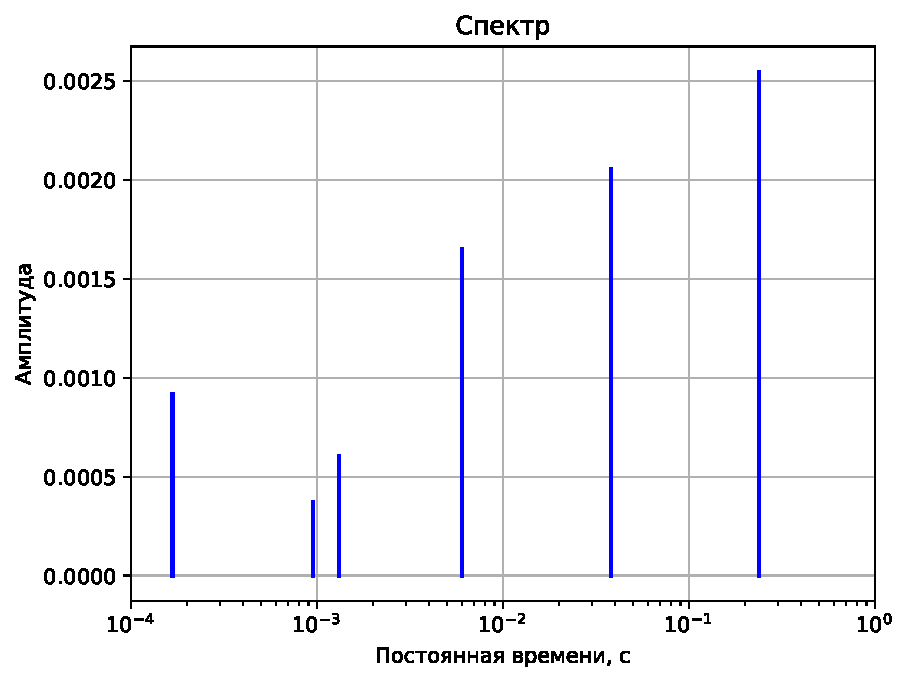
\includegraphics[width=0.5\textwidth]{1564ЛЕ1№1_п1_2500Гц-1Гц_1пФ_+10С_-4В-5В_50мВ_10мкс_шаг_0,01_multi_exp_spectr}
		\caption{Спектр сигнала релаксации ёмкости.}
		\label{pic:multi_exp_spectr_283}
	\end{figure}


	\newpage
	\subsubsection{Сравнение результатов}
	В таблице \ref{table:model_comparison_283} представлено сравнение результатов
	оценки точности рассмотренных моделей. 

	Модель идеального частотного скана демонстрирует значительные отклонения от
	результатов измерений, и, скорее всего, не подходит для описания экспериментальных
	данных, в то время как модель с показателем $p$ и многоэкспоненциальная модель
	неплохо согласуются с результатами измерений и показывают примерно одинаковую
	точность. 
	
	\begin{table}[!htp]
	\centering
	\caption{Результаты идентификации моделей.}
	\begin{tabular}{|l|l|l|}
		\hline
		Модель                    & Результат         & RMSE, пФ \\ 
		                          & кросвалидации, пФ &          \\ \hline
		Идеаьный частотный скан   & 0.001396          & 0.001389 \\ \hline
		Модель с показателем $p$  & 0.000160          & 0.000161 \\ \hline
		Многоэкспоененциальная    & 0.000158          & 0.000156 \\
		модель                    &                   &          \\ \hline
	\end{tabular}
	\label{table:model_comparison_283}
	\end{table}



	\newpage
	\subsection{Частотный скан при температуре 303 К}
	\subsubsection{Моноэкспоненциальная модель с показателем $p$}
	Результаты измерений при температуре 303~К приведены на рисунке 
	\ref{pic:train_data_303}. К сожалению, частотный скан содержит всего 34 точки,
	поэтому гистограммы и графики отклонений будут не так информативны как в 
	предыдущих разделах. Результаты идентификации моноэкспоненциальной модели 
	с показателем $p$ приведены на рисунке \ref{pic:model_single_exp_303}.

	\begin{figure}[!htp]
		\centering
		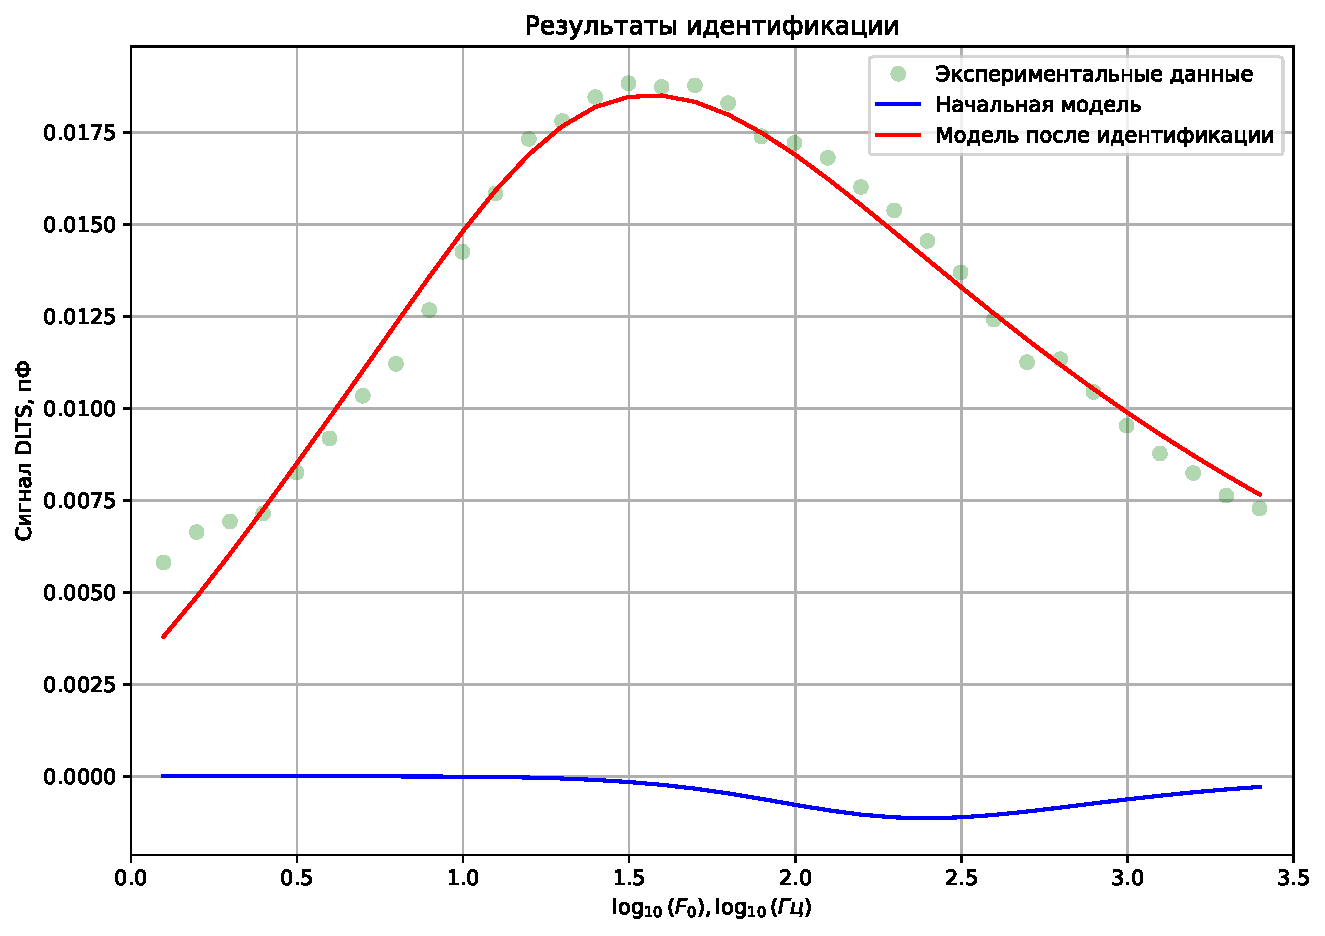
\includegraphics[width=0.75\textwidth]{1564ЛЕ1№1_п1_2500Гц-1Гц_10пФ_+30С_-4В-5В_50мВ_10мкс_шаг_0,1_single_exp_model}
		\caption{Результат идентификации положительного пика частотного скана
		         при $T=303K$.}
		\label{pic:model_single_exp_303}
	\end{figure}

	График нормированной среднеквадратической ошибки, приведенный на рисунке
	\ref{pic:loss_single_exp_303}, указывает на то, что алгоритм идентификации
	нашёл минимум функции потерь.

	\begin{figure}[!htp]
		\centering
		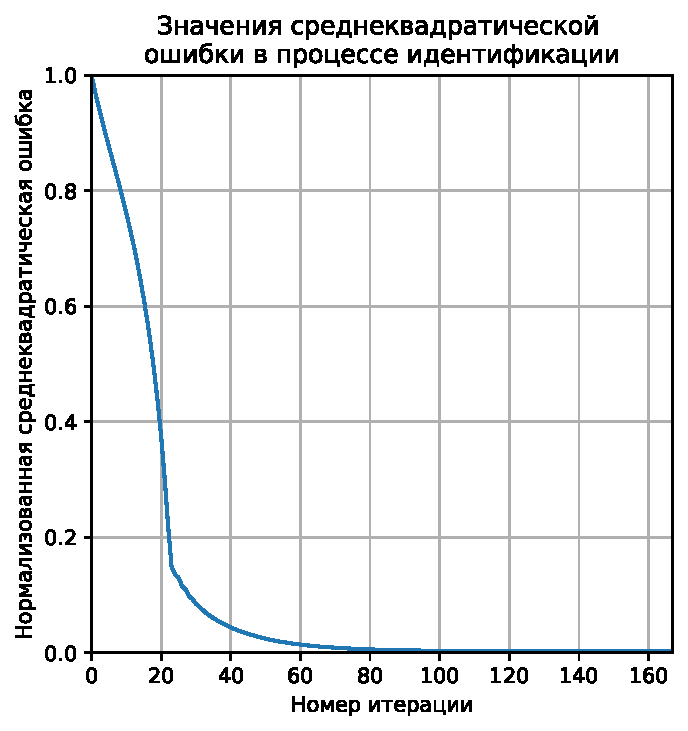
\includegraphics[width=0.35\textwidth]{1564ЛЕ1№1_п1_2500Гц-1Гц_10пФ_+30С_-4В-5В_50мВ_10мкс_шаг_0,1_single_exp_model_loss}
		\caption{График среднеквадратической ошибки в процессе идентификации,
		         нормированной относительно её максимального значения.}
		\label{pic:loss_single_exp_303}
	\end{figure}

	На графике отклонений результатов моделирования, полученных на идентифицированной
	модели, от экспериментальных данных (рисунок \ref{pic:deviations_single_exp_303})
	заметны систематические отклонения. Гистограмма отклонений, приведённая на 
	рисунке \ref{pic:hist_single_exp_303}, по форме существенно отличается от
	нормального распределения.

	\begin{figure}[!htp]
		\centering
		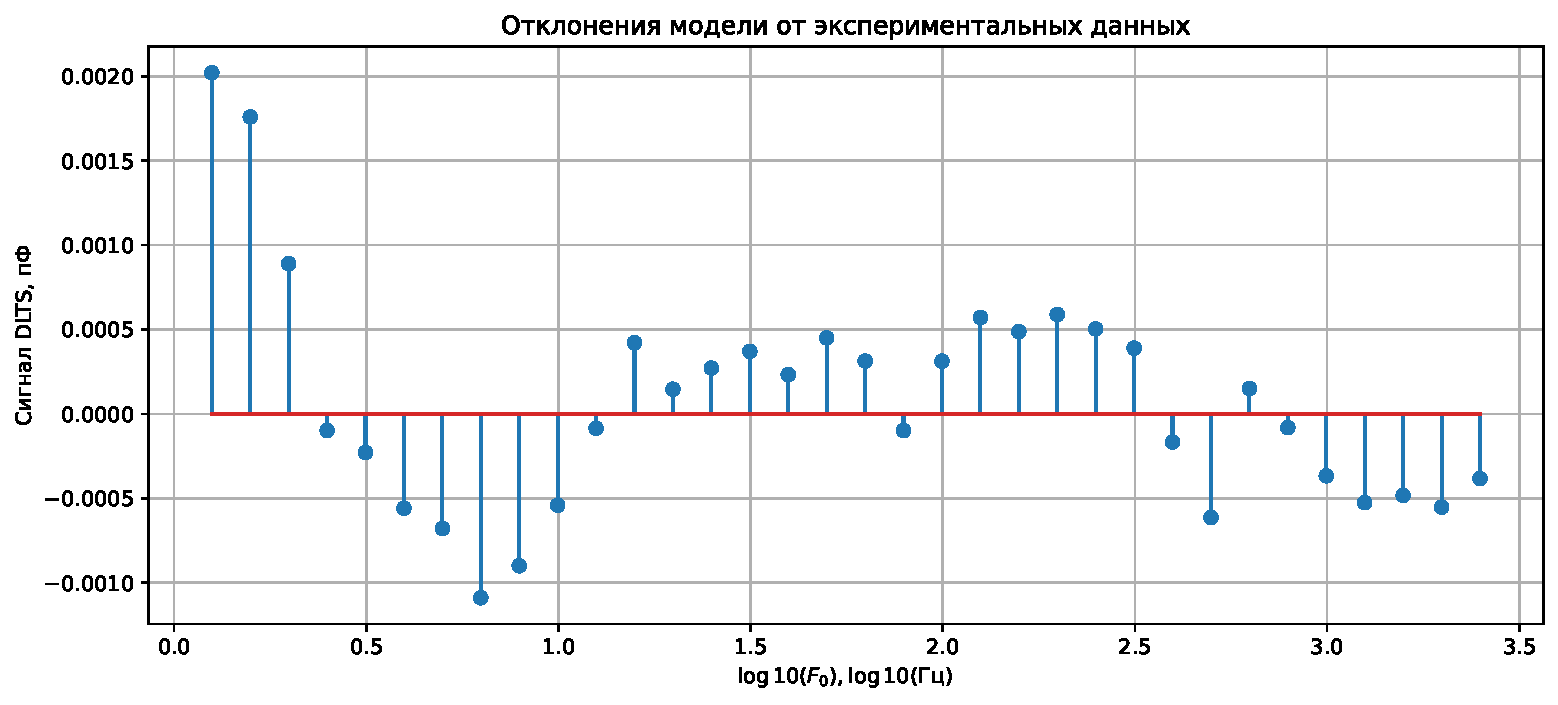
\includegraphics[width=0.75\textwidth]{1564ЛЕ1№1_п1_2500Гц-1Гц_10пФ_+30С_-4В-5В_50мВ_10мкс_шаг_0,1_single_exp_deviations}
		\caption{График отклонений результатов, полученных на идентифицированной
		модели, от экспериментальных данных.}
		\label{pic:deviations_single_exp_303}
	\end{figure}

	\begin{figure}[!htp]
		\centering
		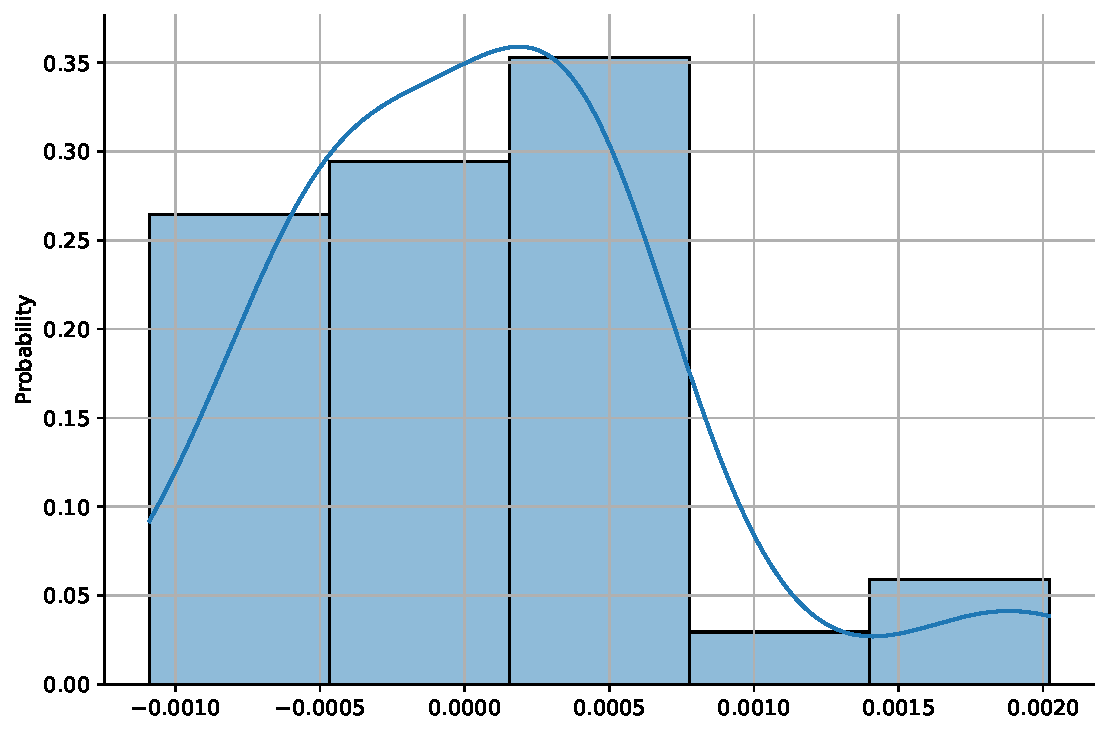
\includegraphics[width=0.5\textwidth]{1564ЛЕ1№1_п1_2500Гц-1Гц_10пФ_+30С_-4В-5В_50мВ_10мкс_шаг_0,1_single_exp_hist}
		\caption{Гистограмма отклонений данных, полученных на идентифицированной 
		         модели, от экспериментальных данных. Сплошной линией показан
		         результат сглаживания гистограммы.}
		\label{pic:hist_single_exp_303}
	\end{figure}

	В таблице \ref{table:results_single_exp_303} приведены параметры 
	идентифицированной модели и результаты оценок точности моделирования.

	\begin{table}[!htp]
		\centering
		\caption{Результаты идентификации модели}
		\begin{tabular}{|l|l|}
			\hline
			Параметр                           & Значение \\ \hline
			Постоянна времени $\tau$, с        & 0,012014 \\ \hline
			Амплитуда, пФ                      & 0.018520 \\ \hline
			Показатель $p$                     & 0.275712 \\ \hline
			Результат кросвалидации (RMSE), пФ & 0.000713 \\ \hline
			RMSE, пФ                           & 0.000660 \\ \hline
		\end{tabular}
		\label{table:results_single_exp_303}
	\end{table}

	На рисунке \ref{pic:spectr_single_exp_303} приведён полученный спектр 
	частотного скана.

	\begin{figure}[!htp]
		\centering
		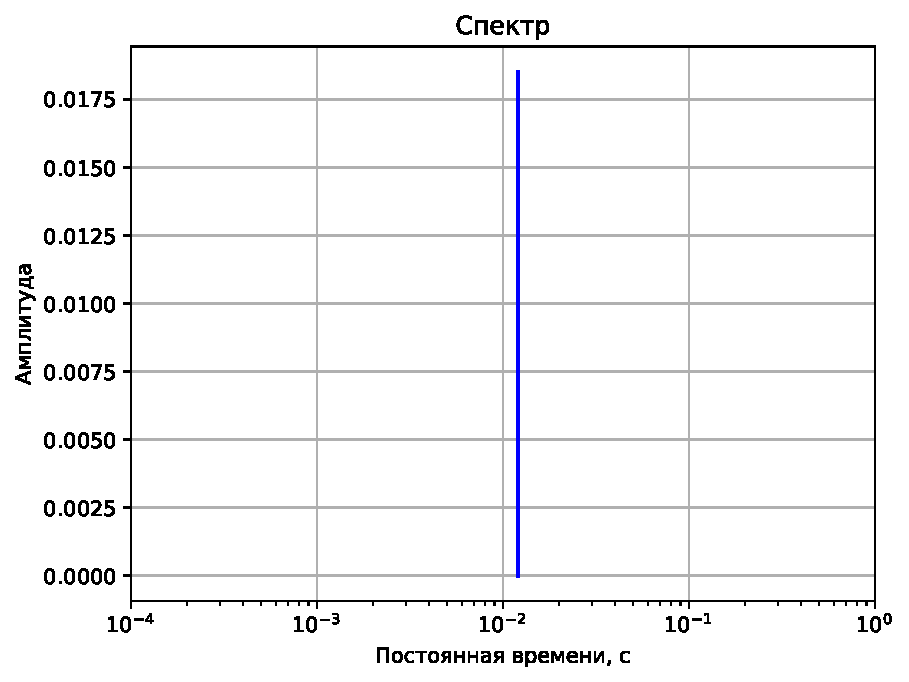
\includegraphics[width=0.5\textwidth]{1564ЛЕ1№1_п1_2500Гц-1Гц_1пФ_+30С_-4В-5В_50мВ_10мкс_шаг_0,01_single_exp_spectr}
		\caption{Спектр сигнала релаксации ёмкости.}
		\label{pic:spectr_single_exp_303}
	\end{figure}


	\newpage
	\subsubsection{Моноэкспоненциальная модель с показателем $p=1$}
	Выполним идентификацию модели идеального частотного скана на результатах,
	полученных при температуре 303~К. Результаты идентификации модели приведены 
	на рисунке \ref{pic:model_single_exp_ideal_303}. На графике заметны
	существенные отклонения результатов моделирования от экспериментальных 
	данных, при этом, график значений нормированной среднеквадратической ошибки
	для каждой итерации (рисунок \ref{pic:loss_single_exp_ideal_303}) 
	свидетельствует о том, что алгоритм идентификации нашёл минимум функции 
	потерь.

	\begin{figure}[!htp]
		\centering
		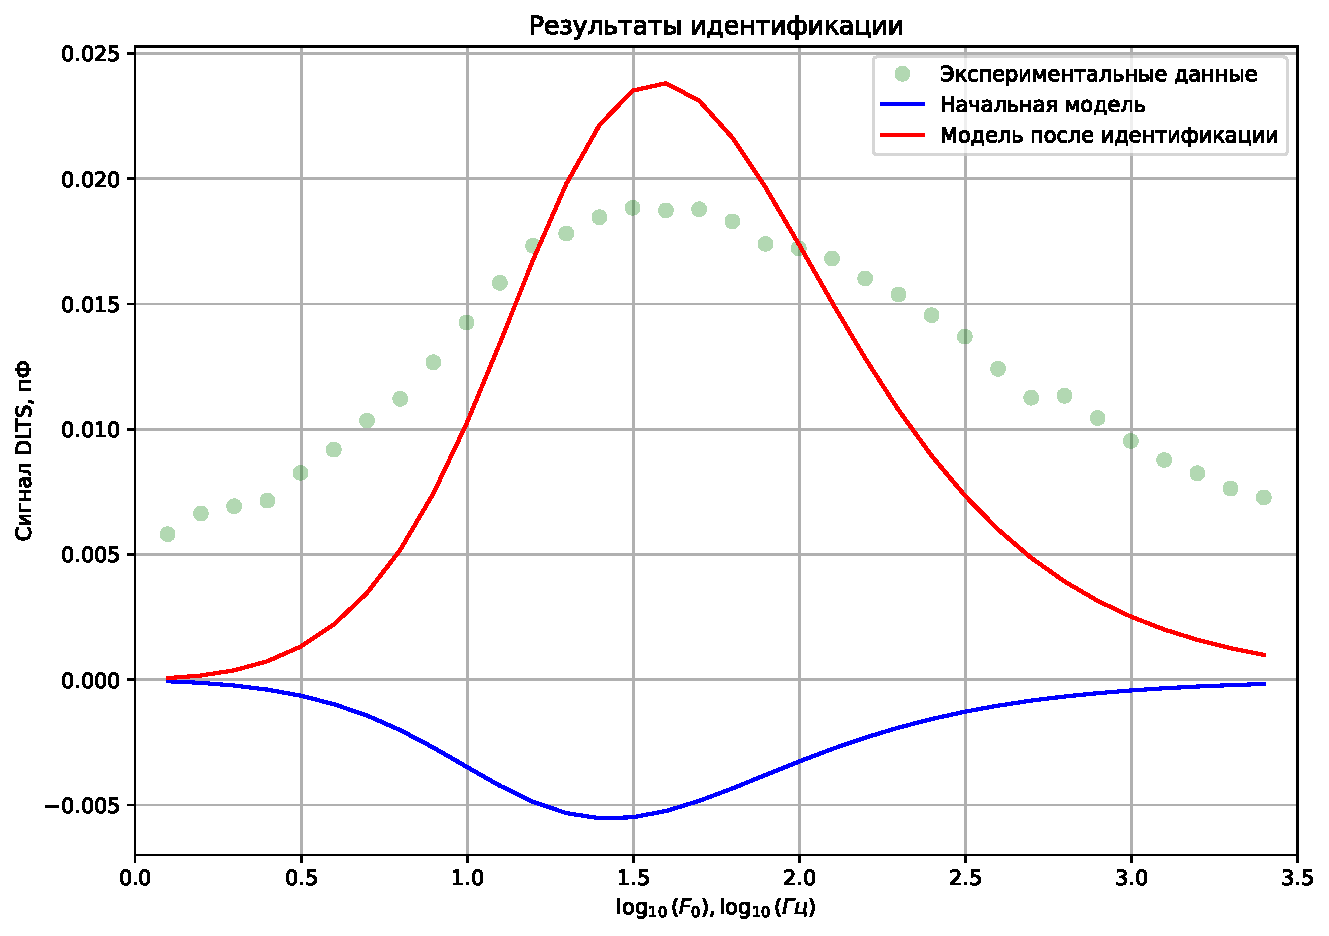
\includegraphics[width=0.75\textwidth]{1564ЛЕ1№1_п1_2500Гц-1Гц_10пФ_+30С_-4В-5В_50мВ_10мкс_шаг_0,1_single_exp_ideal_model}
		\caption{Результат идентификации положительного пика частотного скана
		         при $T=303K$.}
		\label{pic:model_single_exp_ideal_303}
	\end{figure}

	\begin{figure}[!htp]
		\centering
		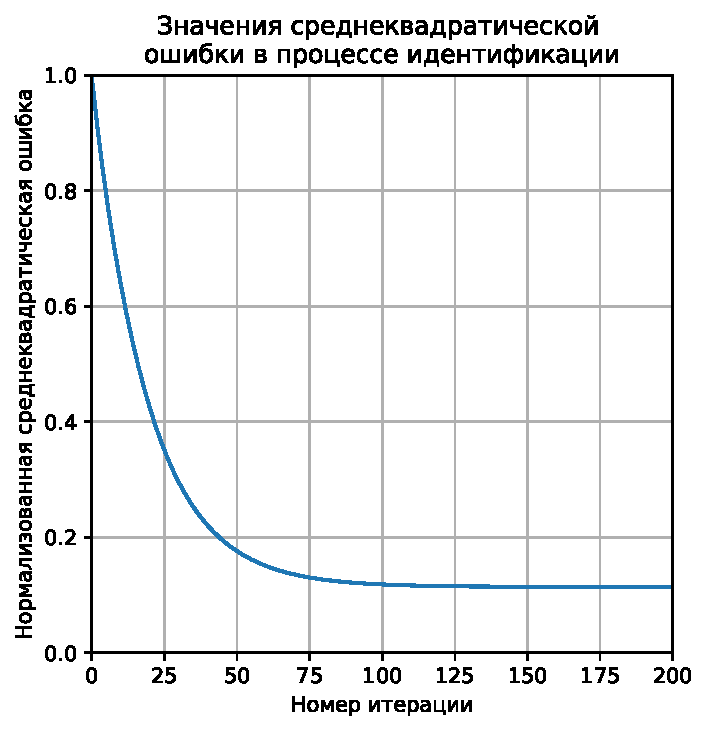
\includegraphics[width=0.35\textwidth]{1564ЛЕ1№1_п1_2500Гц-1Гц_10пФ_+30С_-4В-5В_50мВ_10мкс_шаг_0,1_single_exp_ideal_model_loss}
		\caption{График среднеквадратической ошибки в процессе идентификации,
		         нормированной относительно её максимального значения.}
		\label{pic:loss_single_exp_ideal_303}
	\end{figure}

	График отклонений результатов моделирования от экспериментальных данных
	(рисунок \ref{pic:deviations_single_exp_ideal_303}) также демонстрирует
	значительные систематические отклонения, а гистограмма (рисунок 
	\ref{pic:hist_single_exp_ideal_303}) по форме далека от нормального 
	распределения.

	\begin{figure}[!htp]
		\centering
		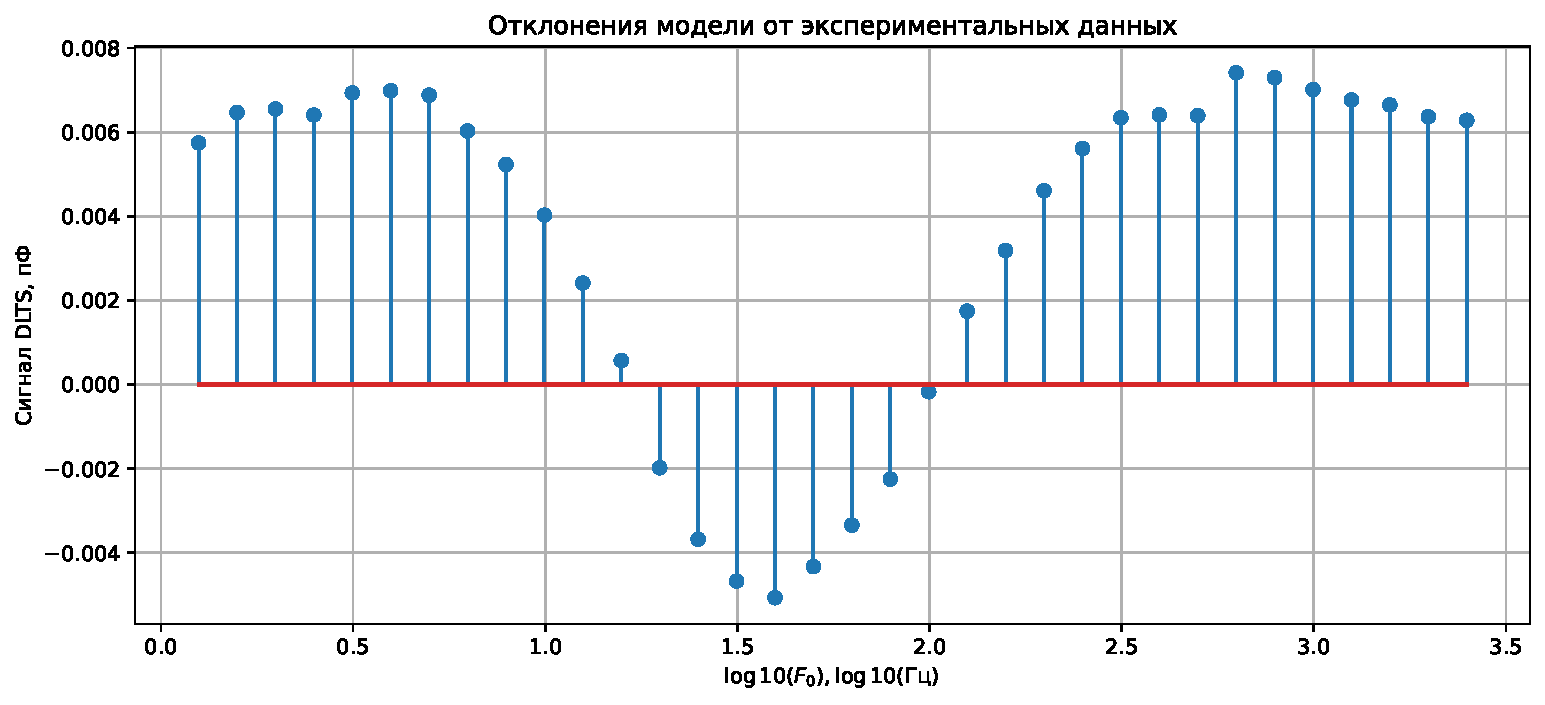
\includegraphics[width=0.75\textwidth]{1564ЛЕ1№1_п1_2500Гц-1Гц_10пФ_+30С_-4В-5В_50мВ_10мкс_шаг_0,1_single_exp_ideal_deviations}
		\caption{График отклонений результатов, полученных на идентифицированной
		модели, от экспериментальных данных.}
		\label{pic:deviations_single_exp_ideal_303}
	\end{figure}

	\begin{figure}[!htp]
		\centering
		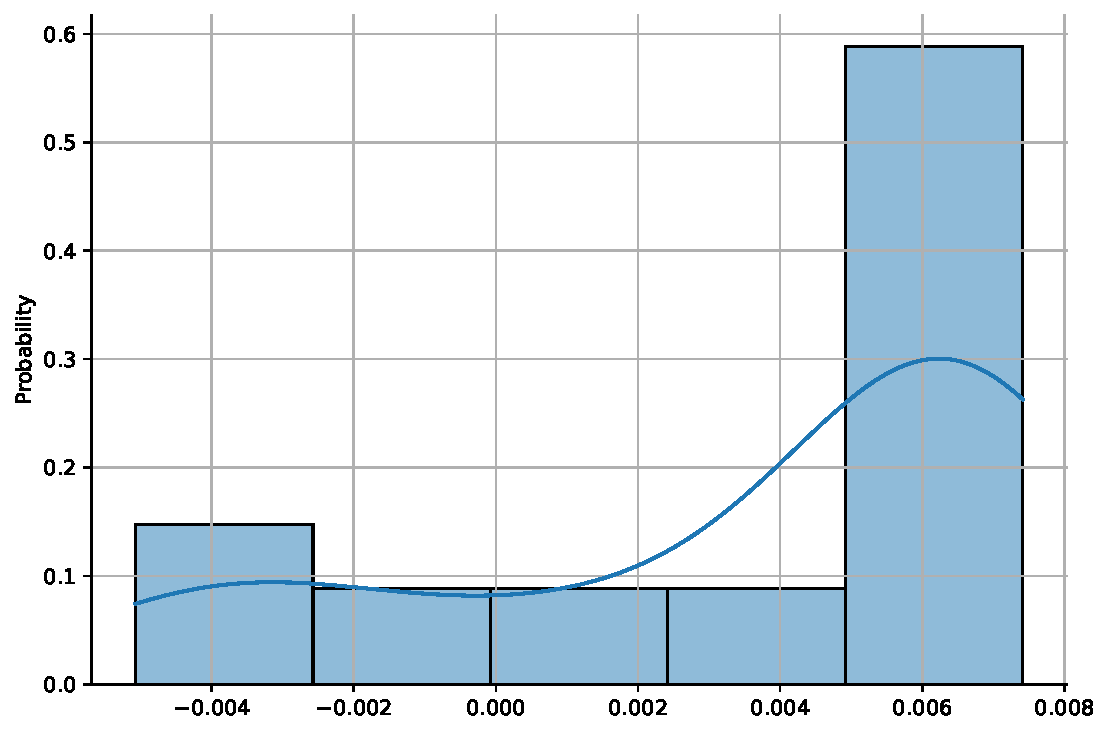
\includegraphics[width=0.5\textwidth]{1564ЛЕ1№1_п1_2500Гц-1Гц_10пФ_+30С_-4В-5В_50мВ_10мкс_шаг_0,1_single_exp_ideal_hist}
		\caption{Гистограмма отклонений данных, полученных на идентифицированной 
		         модели, от экспериментальных данных.Сплошной линией показан
		         результат сглаживания гистограммы.}
		\label{pic:hist_single_exp_ideal_303}
	\end{figure}

	В таблице \ref{table:results_single_exp_ideal_303} приведены параметры 
	идентифицированной модели и результаты оценок точности моделирования.

	\begin{table}[!htp]
		\centering
		\caption{Результаты идентификации модели}
		\begin{tabular}{|l|l|}
			\hline
			Параметр                           & Значение \\ \hline
			Постоянна времени $\tau$, с        & 0,011709 \\ \hline
			Амплитуда, пФ                      & 0.023837 \\ \hline
			Показатель $p$                     & 1.0      \\ \hline
			Результат кросвалидации (RMSE), пФ & 0.005837 \\ \hline
			RMSE, пФ                           & 0.005436 \\ \hline
		\end{tabular}
		\label{table:results_single_exp_ideal_303}
	\end{table}

	На рисунке \ref{pic:spectr_single_exp_ideal_303} приведён полученный спектр
	частотного скана.

	\begin{figure}[!htp]
		\centering
		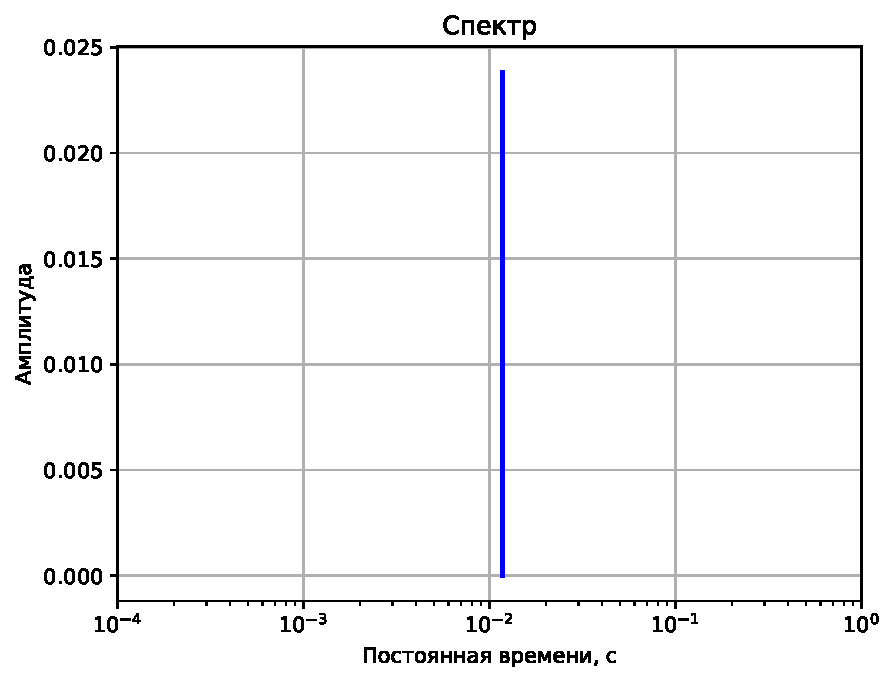
\includegraphics[width=0.5\textwidth]{1564ЛЕ1№1_п1_2500Гц-1Гц_10пФ_+30С_-4В-5В_50мВ_10мкс_шаг_0,1_single_exp_ideal_spectr}
		\caption{Спектр сигнала релаксации ёмкости.}
		\label{pic:spectr_single_exp_ideal_303}
	\end{figure}


	\newpage
	\subsubsection{Многоэкспоненциальная модель с n\_exps > 1}
	Выполним идентификацию многоэкспоненциальной модели, для этого сравним
	результаты кросвалидации для моделей, имеющих значения парамера n\_exps
	равные 5, 6, 7, 8, 9 и 10, и выберем показавшую лучший результат. В таблице
	\ref{table:multi_exp_model_303_cross_val} представлены полученные результаты.
	Лучшей оказалась модель с параметром n\_exps = 6, то есть имеющая 6 
	экспоненциальных составляющих.

	\begin{table}[!htp]
		\centering
		\caption{Результаты кросвалидации для разных значений параметра n\_exps}
		\begin{tabular}{|l|l|}
		\hline
		Значение параметра n\_exps & Результат кросвалидации \\ \hline
		5                          & 0.0005614               \\ \hline
		6                          & 0.0003977               \\ \hline
		7                          & 0.0004187               \\ \hline
		8                          & 0.0004464               \\ \hline
		9                          & 0.0004572               \\ \hline
		10                         & 0.0004476               \\ \hline
		\end{tabular}
		\label{table:multi_exp_model_303_cross_val}
	\end{table}

	Результаты идентификации модели с шестью экспоненциальными составляющими
	представлены на рисунке \ref{pic:multi_exp_model_303}.

	\begin{figure}[!htp]
		\centering
		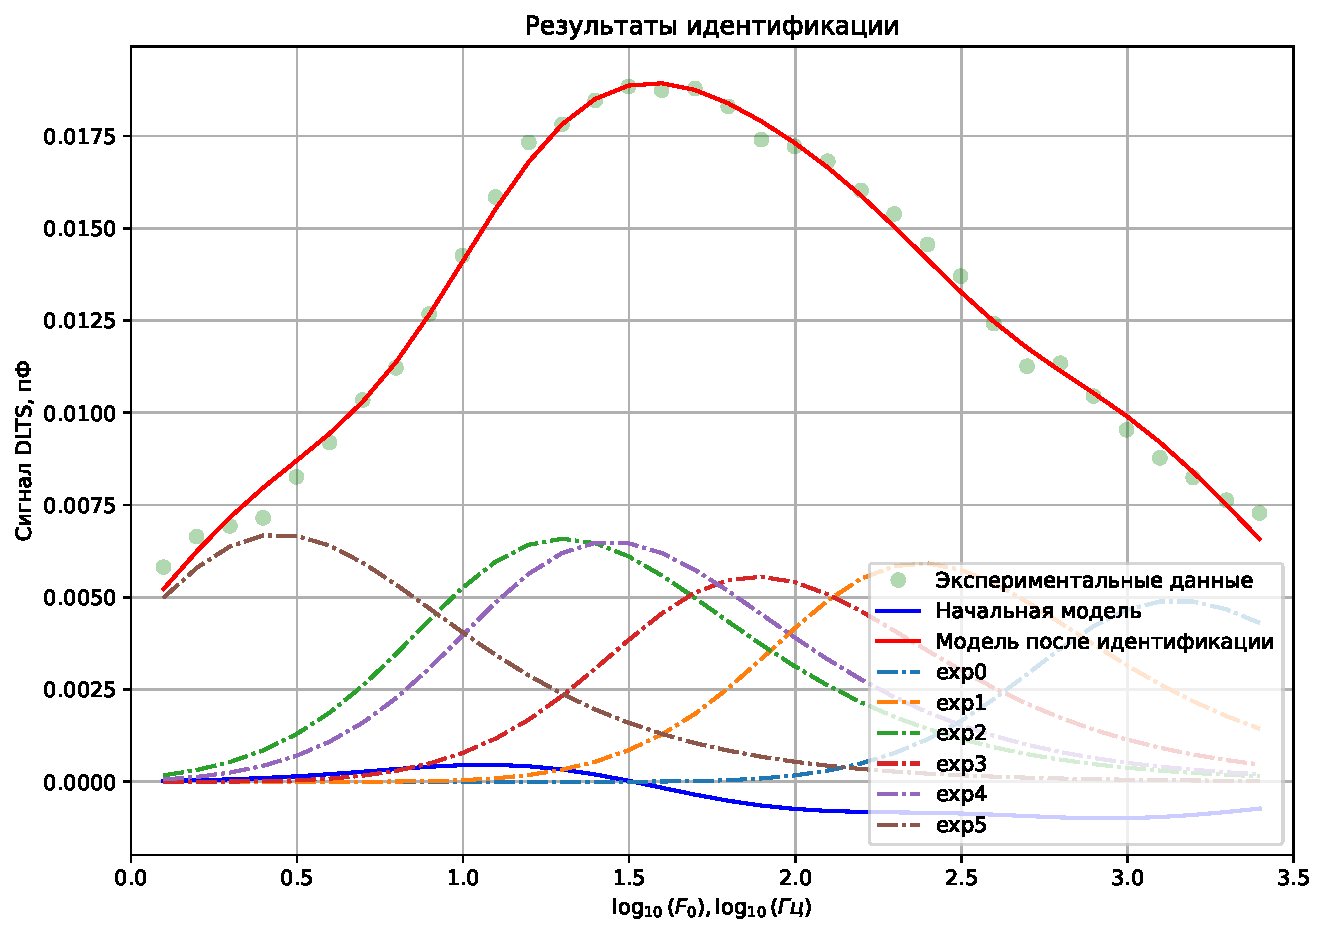
\includegraphics[width=0.75\textwidth]{1564ЛЕ1№1_п1_2500Гц-1Гц_10пФ_+30С_-4В-5В_50мВ_10мкс_шаг_0,1_multi_exp_model}
		\caption{Результат идентификации многоэкспоненциальной моделью 
		         частотного скана при $T=303K$.}
		\label{pic:multi_exp_model_303}
	\end{figure}

	На рисунке \ref{pic:multi_exp_loss_303} показан график нормированной 
	среднеквадратической ошибки. Форма графика говорит о том, что алгоритм
	идентификации нашёл минимум функции потерь.

	\begin{figure}[!htp]
		\centering
		\includegraphics[width=0.35\textwidth]{1564ЛЕ1№1_п1_2500Гц-1Гц_10пФ_+30С_-4В-5В_50мВ_10мкс_шаг_0,1_multi_exp_loss}
		\caption{График среднеквадратической ошибки в процессе идентификации,
		         нормированной относительно её максимального значения.}
		\label{pic:multi_exp_loss_303}
	\end{figure}

	Из-за малого количества точек на частотном скане по графику отклонений
	результатов моделирования от экспериментальных данных (рисунок 
	\ref{pic:multi_exp_deviations_303}) трудно сделать какие-либо выводы.
	Гистограмма отклонений (рисунок \ref{pic:multi_exp_hist_303}) по форме ближе 
	к нормальному распределения, однако, из-за недостаточного количества данных
	не является показательной.

	\begin{figure}[!htp]
		\centering
		\includegraphics[width=0.75\textwidth]{1564ЛЕ1№1_п1_2500Гц-1Гц_10пФ_+30С_-4В-5В_50мВ_10мкс_шаг_0,1_multi_exp_deviations}
		\caption{График отклонений результатов, полученных на идентифицированной
		модели, от экспериментальных данных.}
		\label{pic:multi_exp_deviations_303}
	\end{figure}

	\begin{figure}[!htp]
		\centering
		\includegraphics[width=0.5\textwidth]{1564ЛЕ1№1_п1_2500Гц-1Гц_10пФ_+30С_-4В-5В_50мВ_10мкс_шаг_0,1_multi_exp_hist}
		\caption{Гистограмма отклонений данных, полученных на идентифицированной 
		         модели, от экспериментальных данных.}
		\label{pic:multi_exp_hist_303}
	\end{figure}

	В таблице \ref{table:multi_exp_results_303} приведены параметры 
	идентифицированной модели и результаты оценок точности моделирования,  
	$\tau$ -- постоянная времени, $A$ -- амплитуда.

	\begin{table}[!htp]
		\centering
		\caption{Результаты идентификации модели.}
		\begin{tabular}{|l|l|l|l|}
			\hline
			Параметр                           & Значение & Параметр  & Значение \\ \hline
			$\tau_1$, с                        & 0.000304 & $A_1$, пФ & 0.004912 \\ \hline
			$\tau_2$, с                        & 0.001845 & $A_2$, пФ & 0.005924 \\ \hline
			$\tau_3$, с                        & 0.021940 & $A_3$, пФ & 0.006586 \\ \hline
			$\tau_4$, с                        & 0.005750 & $A_4$, пФ & 0.005556 \\ \hline
			$\tau_5$, с                        & 0.015893 & $A_5$, пФ & 0.006504 \\ \hline
			$\tau_6$, с                        & 0.158127 & $A_6$, пФ & 0.006706 \\ \hline
			Результат кросвалидации (RMSE), пФ & 0.000442 &           &          \\ \hline
			RMSE, пФ                           & 0.000338 &           &          \\ \hline
		\end{tabular}
		\label{table:multi_exp_results_303}
	\end{table}

	На рисунке \ref{pic:multi_exp_spectr_303} приведён полученный спектр 
	частотного скана.

	\begin{figure}[!htp]
		\centering
		\includegraphics[width=0.5\textwidth]{1564ЛЕ1№1_п1_2500Гц-1Гц_10пФ_+30С_-4В-5В_50мВ_10мкс_шаг_0,1_multi_exp_spectr}
		\caption{Спектр сигнала релаксации ёмкости.}
		\label{pic:multi_exp_spectr_303}
	\end{figure}


	\newpage
	\subsubsection{Сравнение результатов}
	В таблице \ref{table:model_comparison_303} представлено сравнение результатов
	оценки точности рассмотренных моделей. 

	Модель идеального частотного скана демонстрирует значительные отклонения от
	результатов измерений, и, скорее всего, не подходит для описания экспериментальных
	данных, в то время как модель с показателем $p$ и многоэкспоненциальная модель
	неплохо согласуются с результатами измерений. Лучшие результаты показывает
	многоэкспоненциальная модель.
	
	\begin{table}[!htp]
	\centering
	\caption{Результаты идентификации моделей.}
	\begin{tabular}{|l|l|l|}
		\hline
		Модель                    & Результат         & RMSE, пФ \\ 
		                          & кросвалидации, пФ &          \\ \hline
		Идеаьный частотный скан   & 0.005837          & 0.005436 \\ \hline
		Модель с показателем $p$  & 0.000713          & 0.000660 \\ \hline
		Многоэкспоененциальная    & 0.000442          & 0.000338 \\
		модель                    &                   &          \\ \hline
	\end{tabular}
	\label{table:model_comparison_303}
	\end{table}


	\newpage
	\subsection{Графики Аррениуса}
	Для завершения анализа и вычисления спектров энергий активации, необходимо
	построить графики Аррениуса. В предыдущем разделе многоэкспоненциальные
	модели для 263~К, 283~К и 303~К имели разное оптимальное количество 
	моноэкспоненциальных составляющих: 8, 6 и 6, соответственно. Для того, чтобы
	было удобнее строить графики в координатах Аррениуса и интерпретировать 
	результаты, выполним повторуную идентификацию всех частотных сканов 
	многоэкспоненциальной моделью с шестью экспоненциальными составляющими.

	Результат идентификации частотного скана при $T=263 K$ и соответствующий
	спектр показаны на рисунках \ref{pic:6_exp_model_263} и 
	\ref{pic:6_exp_spectr_263} соответственно.

	\begin{figure}[!htp]
		\centering
		\includegraphics[width=0.75\textwidth]{1564ЛЕ1№1_п1_2500Гц-1Гц_1пФ_-10С_-4В-5В_10мВ_10мкс_шаг_0,01_6_exp_model}
		\caption{Результат идентификации многоэкспоненциальной модели на 
		частотном скане, полученном при $T=263 K$.}
		\label{pic:6_exp_model_263}
	\end{figure}

	\begin{figure}[!htp]
		\centering
		\includegraphics[width=0.5\textwidth]{1564ЛЕ1№1_п1_2500Гц-1Гц_1пФ_-10С_-4В-5В_10мВ_10мкс_шаг_0,01_6_exp_spectr}
		\caption{Спектр сигнала релаксации ёмкости при $T=263 K$.}
		\label{pic:6_exp_spectr_263}
	\end{figure}



	Результат идентификации частотного скана при $T=283 K$ и соответствующий
	спектр показаны на рисунках \ref{pic:6_exp_model_283} и 
	\ref{pic:6_exp_spectr_283} соответственно.

	\begin{figure}[!htp]
		\centering
		\includegraphics[width=0.75\textwidth]{1564ЛЕ1№1_п1_2500Гц-1Гц_1пФ_+10С_-4В-5В_50мВ_10мкс_шаг_0,01_6_exp_model}
		\caption{Результат идентификации многоэкспоненциальной модели на 
		частотном скане, полученном при $T=283 K$.}
		\label{pic:6_exp_model_283}
	\end{figure}

	\begin{figure}[!htp]
		\centering
		\includegraphics[width=0.5\textwidth]{1564ЛЕ1№1_п1_2500Гц-1Гц_1пФ_+10С_-4В-5В_50мВ_10мкс_шаг_0,01_6_exp_spectr}
		\caption{Спектр сигнала релаксации ёмкости при $T=283 K$.}
		\label{pic:6_exp_spectr_283}
	\end{figure}



	Результат идентификации частотного скана при $T=303 K$ и соответствующий
	спектр показаны на рисунках \ref{pic:6_exp_model_303} и 
	\ref{pic:6_exp_spectr_303} соответственно.

	\begin{figure}[!htp]
		\centering
		\includegraphics[width=0.75\textwidth]{1564ЛЕ1№1_п1_2500Гц-1Гц_10пФ_+30С_-4В-5В_50мВ_10мкс_шаг_0,1_6_exp_model}
		\caption{Результат идентификации многоэкспоненциальной модели на 
		частотном скане, полученном при $T=303 K$.}
		\label{pic:6_exp_model_303}
	\end{figure}

	\begin{figure}[!htp]
		\centering
		\includegraphics[width=0.5\textwidth]{1564ЛЕ1№1_п1_2500Гц-1Гц_10пФ_+30С_-4В-5В_50мВ_10мкс_шаг_0,1_6_exp_spectr}
		\caption{Спектр сигнала релаксации ёмкости при $T=303 K$.}
		\label{pic:6_exp_spectr_303}
	\end{figure}

	Графики в координатах Аррениуса...

	\begin{figure}[!htp]
		\centering
		\includegraphics[width=0.5\textwidth]{arrhenius_lin_regr_with_inset}
		\caption{График в координатах Аррениуса с графиками линейной регрессии}
		\label{pic:arrhenius_lin_regr_with_inset}
	\end{figure}

	\begin{figure}[!htp]
		\centering
		\includegraphics[width=0.5\textwidth]{arrhenius_poly_regr_with_inset}
		\caption{График в координатах Аррениуса с графиками регрессии
		         полиномом второй степени.}
		\label{pic:arrhenius_poly_regr_with_inset}
	\end{figure}